\chapter{LiveClips: Contextual Recommendation of Inspirational Clips from Live Streamed Videos}
\label{chapter:liveclips}
\begin{quote}
Tutorials are helpful for accomplishing specific goals, but people do not always have a particular outcome in mind when using creative software -- sometimes users seek resources for general learning or inspiration. One such resource is live streamed videos, where artists share a window into their creative process. This chapter explores the benefits and challenges of using such videos for learning and inspiration.
%Through content analysis of live stream archives, interviews with 8 streamers, and online surveys with 165 viewers, we study current practices and challenges in creative live stream communities and compare them with prior observations of live streaming in other domains. We observed four common types of creative live streams: teaching, making, socializing, and performing. 
We find that despite the wealth of expert knowledge in live stream archives, their length and volume makes them hard to search or browse. To address this challenge, we introduce \textit{LiveClips}: a system for automatically selecting inspirational segments from live streamed videos and recommending them to users in the context of their creative workflows. We present three methods for recommending and displaying video clips with varying levels of contextual support, and implement them in a popular creative application, Adobe Photoshop. We compare the accuracy of LiveClips' clip ranking to human ranking and present initial user feedback on the three prototypes.
\end{quote}

\section{Introduction}
Browsing and exploring inspiring examples is a key part of the creative process \cite{Shneiderman2007, Shneiderman2002, Greene2002, Herring2009, Bawden1986}. Prior work has shown that seeing examples throughout the entire process, including the beginning, middle, and even towards the end, is valuable~\cite{Kulkarni, Siangliulue2015}. One popular source for creative examples is online communities such as 500px, Behance and Dribbble\footnote{\url{500px.com}, \url{behance.net}, \url{dribbble.com}}. However, these tend to showcase finished projects, which give the viewers little to no insight about \textit{how} or \textit{why} a project was created. 

Recent work has shown that seeing the process behind an artist's work is beneficial for creativity, as it encourages self-reflection on one's own process and methods \cite{Kim2017}. An increasingly popular way to share process (not only for creative work, but also other domains such as gaming) is live-streaming through platforms like Twitch and YouTube\footnote{\url{twitch.tv}, \url{youtube.com}}. Many artists working with both digital and physical tools live-stream as they work on a project (e.g., graphic design, drawing). As a result, there is a rapidly growing collection of archived live-stream videos that contain both inspirational and educational content regarding artists' creative processes. However, finding moments that are relevant and personally inspiring to a creator from this large collection of videos can be difficult, making live-streams an under-utilized source for potential examples.

This work introduces RePlay, a system for automatically selecting good segments from long live-streamed videos and recommending them as examples to users in the context of their creative workflow. We choose to present examples inside the user's software in an effort to make examples more available throughout the entire creative process.
%based on the known benefits of contextual in-application learning \cite{Grossman2010a, Pongnumkul2011, Kelleher2005, Dontcheva2014}. 
Contextually available examples increase the likelihood of unexpected, or ``serendipitous'' discoveries, which research has shown can spark new ideas in a wide range of creative domains, such as scientific research, writing, and visual art \cite{Bawden1986, Benjamin2014, Foster2003, Erdelez1999}. RePlay's goal is to make examples pervasive in the creative process, to promote and encourage serendipitous moments of inspiration. 

RePlay combines telemetry and computer vision techniques to automatically segment long videos into short 25-second clips, crop clips intelligently to a thumbnail size for easy viewing, and recommend clips to creative software users based on their usage behaviour. We demonstrate RePlay's method by using it to automatically extract and rank clips from 17 live-streamed videos of artists working in two popular creative applications, Adobe Photoshop and Illustrator. We focus on digital art tasks such as design and illustration, as these are currently popular tasks for live-streaming, and the software used for these tasks has wide audiences.

We compare RePlay's ranking algorithm to human ranking and find that RePlay is able to predict a clip's inspirational value with reasonable accuracy. To demonstrate how short inspirational clips can be contextually embedded in creative software, we present a design space and three prototypes that lie within this space, implemented in Adobe Photoshop (\autoref{fig:liveclips_photoshop}). Initial user feedback suggests that this approach is promising and warrants further study. In summary, we make the following contributions:

\begin{itemize}
\item a formative understanding of creative software live-streams based on user surveys and video analysis,
\item a method for extracting short (25-second) clips from long live-streamed videos and cropping them to thumbnail size,
\item an approach for selecting example clips to present inside creative software based on their visual properties, the user's tool usage, and the presentation location within the software,
\item three prototype implementations in a creative application and validation of the ranking approach with human raters. 
\end{itemize}

\section{Related Work}
Supporting inspiration and creativity is difficult to study because the unpredictable nature of inspiration makes it hard to quantify \cite{Shneiderman2007}. However, prior research agrees that supporting exploratory search and the gathering of examples is a key attribute for tools that aim to stimulate creativity \cite{Shneiderman2007, Shneiderman2002, Muller-Wienbergen2011, Greene2002, Bawden1986}. Creative work today often involves combining preexisting works in novel ways \cite{Benjamin2014}, or drawing new connections between seemingly disparate things \cite{Foster2003}. While inspiration can stem from just about anywhere, in this work we focus on examples of others' work, a proven source for creative inspiration \cite{Benjamin2014, Foster2003}.

\subsection{Examples are important for creative inspiration}
Searching and browsing examples is an important part of the creative process \cite{Shneiderman2002, Shneiderman2007, Greene2002, Herring2009, Muller-Wienbergen2011, Bawden1986}. 
While search engines are a common tool for finding examples, directed search can prevent serendipitous discovery \cite{Benjamin2014}. Happening upon an unexpected or even seemingly unrelated example can spark new ideas that the creator wouldn't have otherwise thought of \cite{Erdelez1999, Benjamin2014}.
Creative software can support serendipitous discovery by presenting the user with examples while they work \cite{Bawden1986, Kulkarni2014, Herring2009}.

The selection of examples is important; prior work shows that diverse and far-ranging examples lead to more novelty in creative output \cite{Chan2011} and more diverse sets of ideas \cite{Siangliulue2015a} than examples that are similar to each other and the task at hand. The timing of examples is also important; Lewis et al. \cite{Lewis2011} show that people can be primed to be more creative through exposure to examples before a creative task, while Kulkarni et al. \cite{Kulkarni2014} show that seeing examples early on in the process as well as interspersed throughout the process improves creativity. However, diverse examples can actually be harmful if they are presented while the user is being productive \cite{Chan2017}. Siangliulue et al. \cite{Siangliulue2015} found that the most novel ideas occur when examples are only shown at the user's request rather than automatically shown by the system. However, users may not always remember to look for examples, and so systems that ambiently update or recommend examples when the user is idle have also shown creative benefits \cite{Siangliulue2015, Rhodes1996}.

RePlay selects a diverse set of examples that are relevant to the user's context. Guided by the research above, our prototype implementations explore variations in the timing and availability of examples.

%\subsection{Inspirational vs. educational content}
%In the context of creative work with software (e.g., design, digital painting), educational content consists of instructions for achieving certain tasks or techniques, learning material for how to use tools in the software, and tips or advice for creating good work (e.g., \cite{Grossman2010a, Pongnumkul2011, Kelleher2005, Chi2012}). Inspiration on the other hand can come from almost anywhere \cite{Cobbledick}, but a prominent type of content for inspiration in research on creativity is examples of others' work \cite{Muller-Wienbergen2011, Shneiderman2002, Herring2009, Kulkarni, Siangliulue2015a, Siangliulue2015}. One key difference therefore between educational and inspirational content is that educational content focuses more on the \textit{technique} behind accomplishing something, whereas inspirational content focuses more on the \textit{content} being created. There can be overlap between these categories; creative live-streams are one example of content that can be both inspirational and educational. Their main focus tends to be on the content the artist is creating, but along the way the artist may also demonstrate specific techniques or mention helpful tips. In this way creative live-streams bridge the gap between learning and inspiration. The next section in this paper discusses the content of creative live-streams in more detail.

\subsection{Embedding contextual recommendations in software}
Given the increased focus in education (e.g., \cite{Prince2004}) and software learning (e.g., \cite{Greene2002, Grossman2010a}) on active learning, or ``learning while doing'', we believe similar benefits may arise by integrating the process of inspiration with the process of doing. Despite the known benefits of seeing examples throughout the creative process \cite{Kulkarni2014}, most creative software tools today lack support for in-context inspiration. Contextual presentation of learning content is an effective method for supporting learning while doing \cite{Grossman2010a, Matejka2011, Ichinco2017, Matejka2009}; in this work we explore whether contextual presentation of examples can similarly support ``inspiration while doing''. 

Embedding any kind of content in-app runs the risk of interrupting or distracting the user. Therefore, in-app content should be unobtrusive but easy to access \cite{Grossman2010a}. Tooltips are one promising avenue for this, as they only require a hover to access and can be easily dismissed by mousing away. Inspired by ToolClips \cite{Grossman2010a}, this work also uses tooltips as one potential interface for contextual assistance. 
%It is also beneficial to include multiple different examples of tool or command use to help users better understand how it works outside of any one particular context \cite{Grossman2010a, Lafreniere2014, Ichinco2017}. 
CommunityCommands, a command recommender for AutoCAD \cite{Matejka2009}, demonstrated that personalizing recommendations based on the user's own tool use makes them more likely to be helpful. Over a 6-week user study of CommunityCommands, Li et al. \cite{Li2011} found that recommendations based on the user's short-term tool use are preferred over those based on the user's all-time tool use, as the former tend to be more contextually relevant. RePlay similarly bases recommendations on the user's recent tool use.

\begin{figure}[b!]
\centering
  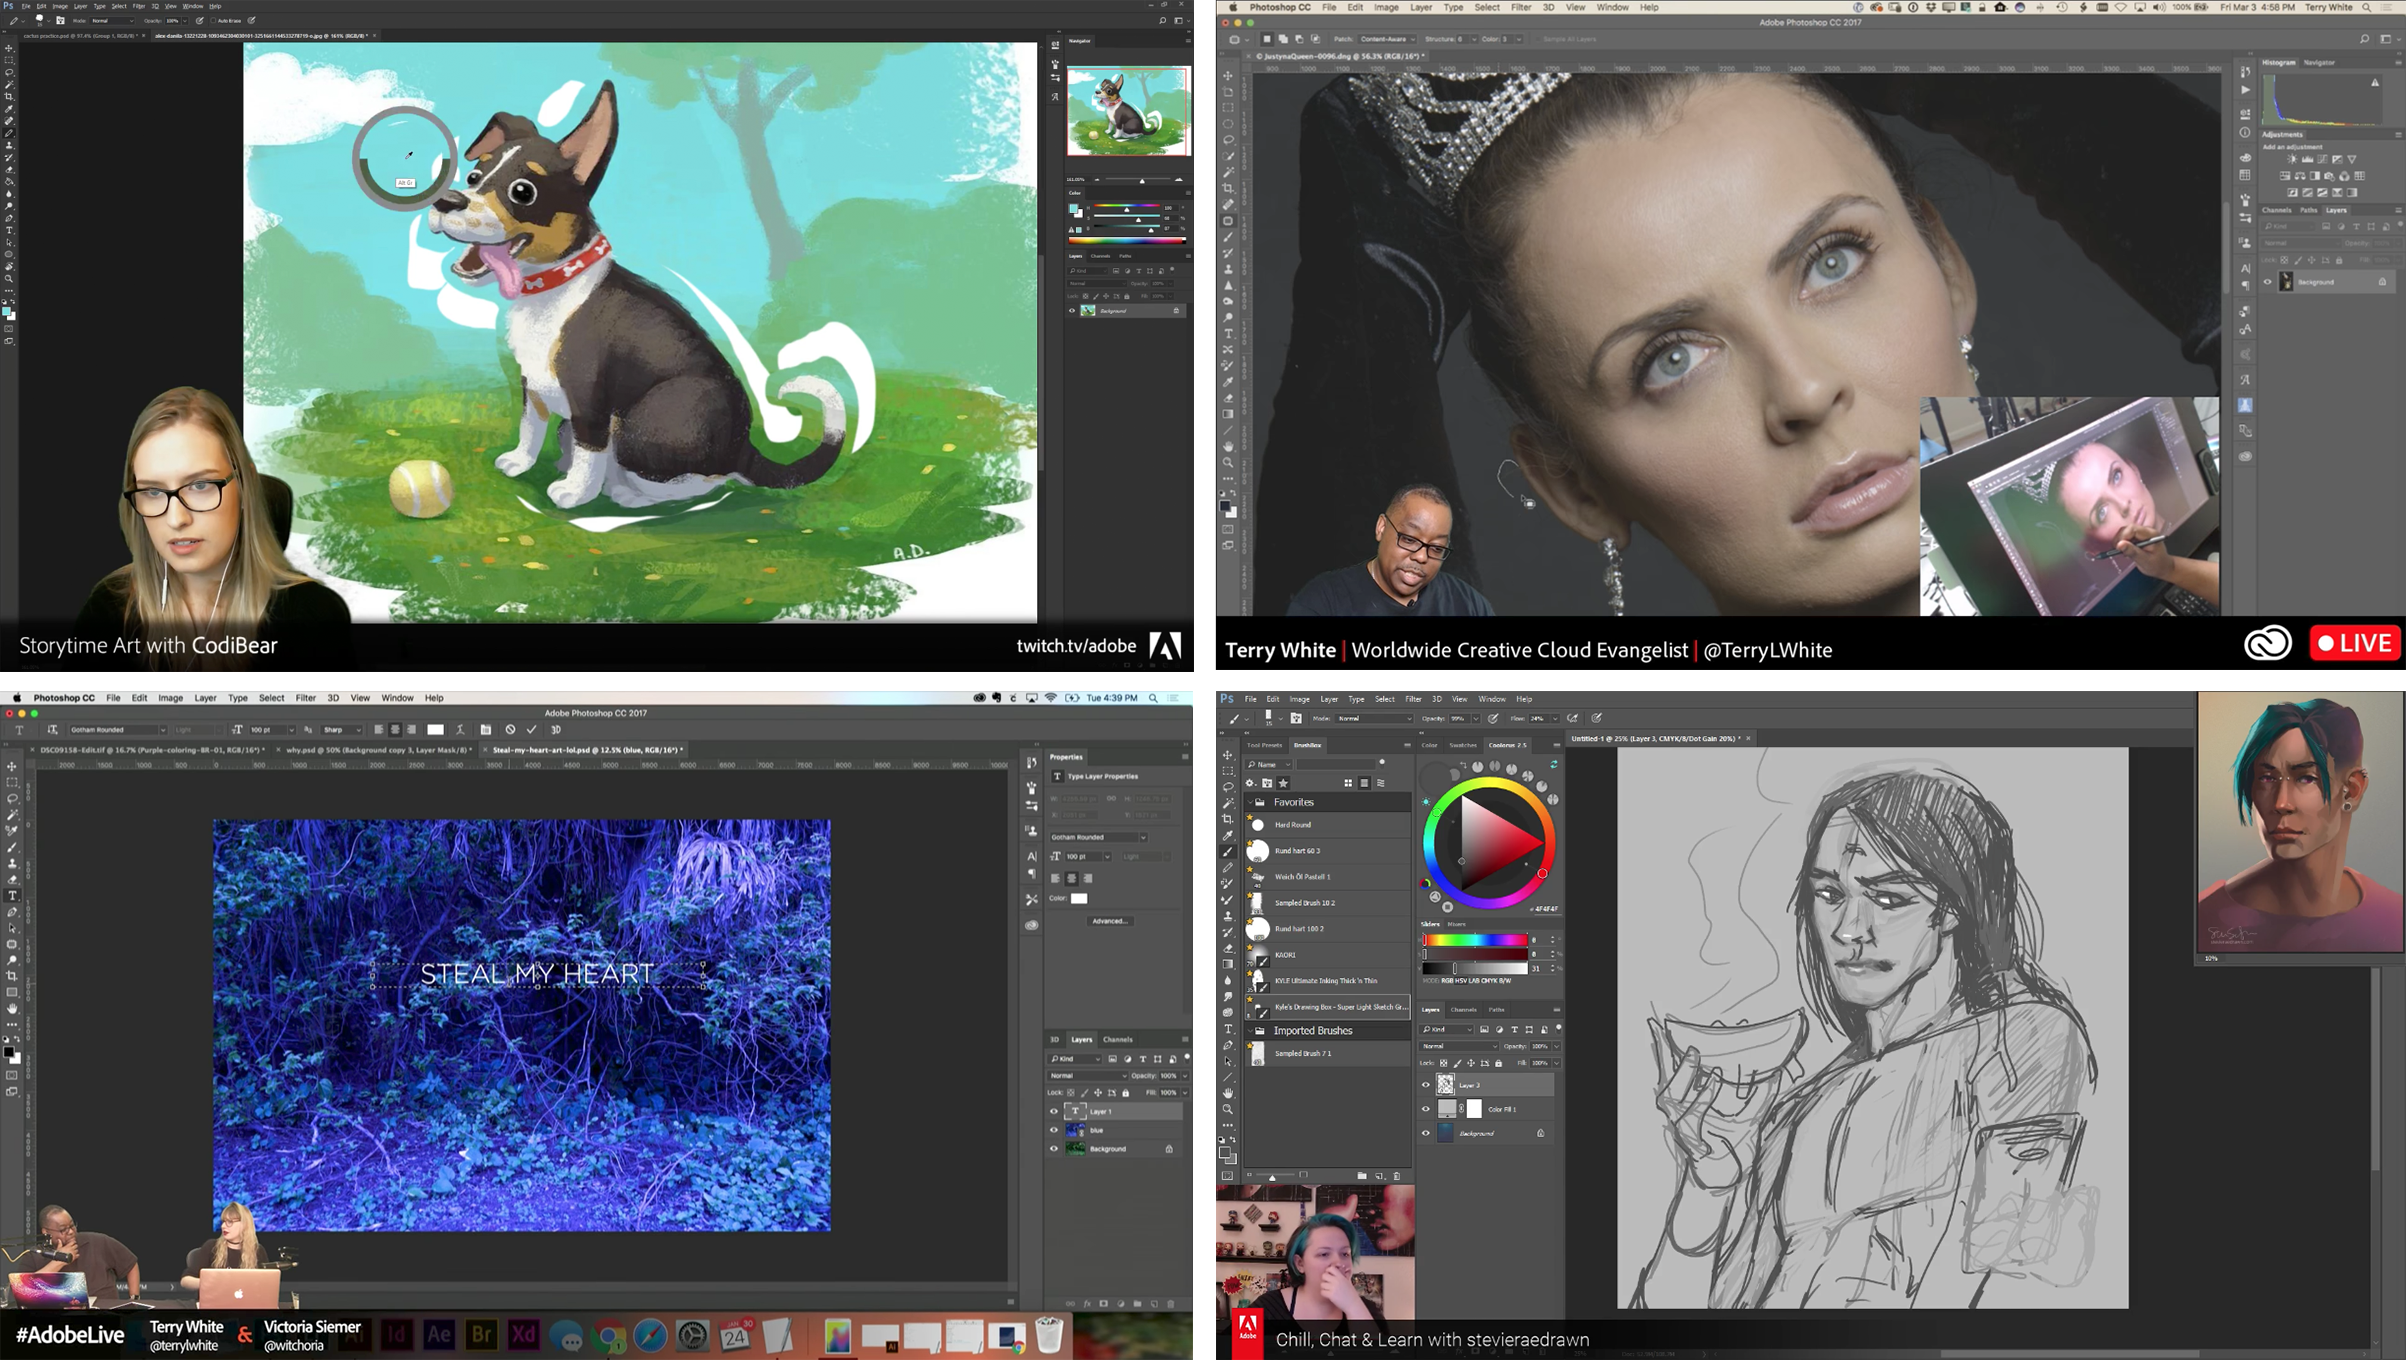
\includegraphics[width=\columnwidth]{liveclips/figures/streamers.png}
  \caption{Examples of creative live-streams on Twitch and YouTube. Artists stream videos of themselves working on creative projects such as graphic design, illustration, and photo editing. (Sources for video screenshots: top left\protect\footnotemark, top right\protect\footnotemark, bottom left\protect\footnotemark, bottom right\protect\footnotemark)}~\label{fig:liveclips_streamers}
\end{figure}

\subsection{Segmenting videos to make them more browsable}
This work uses videos as the source for inspirational examples. Videos have the advantage over text and static images that they show the process of using a tool, rather than just the outcome, and they provide visual demonstrations that are directly relatable to the visual user interface \cite{Grossman2010a}.

Extensive prior work has explored automatically generating educational video clips from screencast videos of software use \cite{Pongnumkul2011, Chi2012, Banovic2012, Lafreniere2014, Nguyen2015}. Though some methods rely on matching telemetry data for these videos \cite{Grossman2010, Lafreniere2014, Chi2012}, others have shown that computer vision alone can be used to detect tool selection events when such data is not available \cite{Pongnumkul2011, Banovic2012}. In this work, we use telemetry data to segment live-streamed videos into clips and rely on computer vision for the presentation and ranking of clips. 

Given a long video with associated tool data, prior work suggests techniques for extracting clips that demonstrate particular tools \cite{Pongnumkul2011, Chi2012, Lafreniere2014}, and guidelines for selecting clips with the best learning value \cite{Lafreniere2014}. Lafreniere et al.'s recommended guidelines \cite{Lafreniere2014} include keeping clips short (15-25 seconds), using clips that show clear visual change to the document, and avoiding clips that show multiple unrelated actions. RePlay builds on this approach to extract and rank clips from live-streamed videos and explores how the characteristics of an inspiring clip might differ from that of an instructional one.

\section{Formative Work: Understanding Creative Live Streams}
\label{sec:liveclips_formative}
Creative live streams are a unique and rapidly growing source of data that have yet to be deeply studied.  To understand the current landscape of creative live streams as well as their applicability to inspiration in software, we conducted content analysis, interviews, and surveys, exploring the following three questions:

\begin{enumerate}
    \item \textbf{What are creative live streams?} For a general sketch of creative live streams, we present a content analysis of a sample of live streams that illustrates the range of content people stream and the different types of creative live streams.
    \item \textbf{Why and how do people stream creative work?} Which parts of their process do they stream? To understand streamers' motivations, processes, and challenges, we present findings from interviews with 8 creative streamers and compare their experiences with streamers in other domains.
    \item \textbf{Why do people watch creative live streams?} To understand the audience these streamers reach, we present findings from three online surveys with 165 viewers that highlight learning and inspiration as key motivators, with entertainment and community close behind.
\end{enumerate}

We found that viewers often seek to learn and be inspired from creative live streams. Notably, inspiration is a much more prominent theme compared with prior work in other live streaming domains such as gaming. However, many streaming platforms are not designed to support these goals, and watching archived streams is tedious. These findings further motivate our goal to make live streams available to users in the context of their own workflows.

\subsection{What Are Creative Live Streams?}
Live stream videos (\autoref{fig:livestreaming_view}) typically show the artist's full screen (when working on a computer) or workspace (for physical work) and a camera view of their face. Live streams usually also feature a live chat, allowing viewers to communicate with each other and the artist. 

There are two main things that make live streamed videos different from other types of videos demonstrating creative work, such as tutorials. First, live streamed videos usually show a real-world process, imparting both creative and procedural knowledge, while tutorials often show contrived tasks, and impart mainly procedural knowledge \cite{Torrey2007}. Second, artists often start without an exact goal in mind, and it can be inspiring to watch someone go from a blank canvas to a beautiful piece of work, though this also means watching the less ``glamorous'' parts of the creative process such as silent thinking or tedious, repetitive tasks.

To learn more about creative live streams, we studied two popular platforms: Twitch and YouTube. As these large platforms cover many types of content, we narrowed our investigation to the \textit{Creative} category on Twitch and the \textit{Adobe Live} video series on YouTube. Through this, we see how streams and communities differ across platforms.  

\begin{figure}[b!]
\centering
  \includegraphics[width=0.7\columnwidth]{liveclips/figures/livestreaming_paper_figure_anonymized.jpg}
  \caption[A typical creative live stream setup.]{A typical creative live stream setup. (a) A camera or screencast displays the artist's workspace. (b) A second camera shows the artist's face. (c) Graphical overlays provide ambient information about the artist (\textit{e.g.}, social media pages) and display interactions with the audience (\textit{e.g.}, pop-ups that appear when viewers subscribe or donate to the stream). (d) Live chat allows viewers to communicate with the streamer. }~\label{fig:livestreaming_view}
\end{figure}

\subsubsection{Creative live streams on Twitch: Content analysis}
To better understand the format and content of creative live\-streams, we analyzed a sample of videos on Twitch, one of the most popular platforms for live streaming. For each creative category, we gathered aggregate metrics about streamers and viewers. We watched and took notes on a sample of 29 videos. We identified four common types of creative live streams that will appear throughout the chapter: \textit{Teaching}, \textit{Making}, \textit{Socializing}, and \textit{Performing}.

\textbf{Methodology:}
To measure the popularity and activity in each of the six creative categories, we queried the Twitch \textsc{api} 4 times a day for 7 days to obtain the number of currently-live streams and number of currently-watching viewers in each category.

We also used the Twitch \textsc{api} to download metadata about the videos in each category (limited to top 600)
%Because this \textsc{api} halts video requests after 600 videos, so our script downloaded metadata for the 600 most-viewed videos in each category. The script 
and randomly selected 50 archived English live stream videos. Four annotators (including the first author) watched each of these videos. Ten videos were not available for viewing and thus excluded (either because their archive expired between being downloaded and being annotated, or because they were only available to subscribers of a channel). Another 11 videos were excluded as they showed video games, TV show reruns, or live event coverage. While these videos were categorized as creative on Twitch, they did not reflect our definition of creative work, namely the creation of a novel artifact. This yielded 29 videos. For each, annotators took notes in a structured spreadsheet on the content presented, camera setup, overall structure of the stream, artist's presentation style, and chat activity.

\begin{table}[t]
\centering
\caption{Summary of popularity of Twitch's creative live stream categories. The number of currently-live streams and currently-watching viewers were collected 4 times a day for a week and then averaged.}~\label{table:livestream_summary}
\begin{tabular}{llll}
\textbf{Category}        & \textbf{\begin{tabular}[c]{@{}l@{}}Avg. \#\\ live streams\end{tabular}} & \textbf{\begin{tabular}[c]{@{}l@{}}Avg. \# live\\ viewers\end{tabular}} & \textbf{\begin{tabular}[c]{@{}l@{}}Avg. \# viewers\\ / stream\end{tabular}} \\
Art                      & 339                                                                    & 6417                                                                    & 21                                                                          \\
Beauty \& Body Art       & 5                                                                      & 177                                                                     & 17                                                                          \\
Food \& Drink            & 19                                                                     & 1088                                                                    & 64                                                                          \\
Makers \& Crafting       & 40                                                                     & 680                                                                     & 16                                                                          \\
Music \& Performing Arts & 286                                                                    & 6881                                                                    & 24                                                                          \\
Science \& Technology    & 91                                                                     & 1155                                                                    & 12                                                                         
\end{tabular}
\end{table}

While this sample does not capture all types of creative activities one might live stream, our hope is that by analyzing a set of canonically creative activities we can shed light on a broader set of activities that might also have a creative component (\textit{e.g.}, video games that involve creating artifacts).
%There is overlap among categories on Twitch, even sometimes within a single live stream when an artist switches back and forth between creative work and other activities like gaming. 

\textbf{Results: Most streamers focus on work \& engage with viewers:}
\autoref{table:livestream_summary} shows overall metrics for the creative categories on Twitch. The most popular categories by far are \textit{Art} and \textit{Music \& Performing Arts}. The category with the most viewers watching per stream is \textit{Food \& Drink}, likely because there are fewer streams to choose from relative to the number of interested viewers. These communities are small relative to the most popular games; for example, the game Fortnite has between 5,000 and 10,000 streams live on Twitch at any given time, with around 100,000 total viewers watching. %\xxx{xxx says move earlier but where?}

\begin{table}[t!]
\centering
\caption{Creative activities shown in a random sample of 29 live streams from Twitch's creative categories, and the primary type of structure each stream exhibits.}~\label{table:livestream_activities}
\begin{tabular}{lll}
\textbf{Category}        & \textbf{Activity (\# videos if \textgreater 1)} & \textbf{\begin{tabular}[t]{@{}l@{}}Primary type\\ of stream\end{tabular}} \\
Art                      & Multimedia production                           & Making                                                                    \\
                         & Digital drawing (4)                             & Making                                                                    \\
                         & Animation                                       & Teaching                                                                  \\
                         &                                                 &                                                                           \\
Beauty \& Body Art       & Makeup                                          & Socializing                                                               \\
                         & Makeup (3)                                      & Making                                                                    \\
                         &                                                 &                                                                           \\
Food \& Drink            & Cooking                                         & Teaching                                                                  \\
                         &                                                 &                                                                           \\
Makers \& Crafting       & Making foam props                               & Teaching                                                                  \\
                         & Sewing quilts                                   & Socializing                                                               \\
                         & Bead art (2)                                    & Making                                                                    \\
                         & Assembling models                               & Making                                                                    \\
                         & Assembling models                               & Socializing                                                               \\
                         & Woodworking                                     & Making                                                                    \\
                         & Pottery                                         & Making                                                                    \\
                         &                                                 &                                                                           \\
Music \& Performing Arts & Music production                                & Performing                                                                \\
                         & Music production                                & Making                                                                    \\
                         & Acting \& improv games                          & Performing                                                                \\
                         &                                                 &                                                                           \\
Science \& Technology    & Building a computer                             & Making                                                                    \\
                         & Programming (3)                                 & Making                                                                    \\
                         & Game development (2)                            & Teaching                                                                  \\
                         & Talking about technology                        & Socializing                                                              
\end{tabular}
\end{table}

The videos span a range of creative activities (\autoref{table:livestream_activities}). The average video length was 3h46m, not including time spent gaming -- a few artists combined both creative work and video gaming into one stream, spending the first part on creative work then switching to gaming when they were finished. The shortest video was 1h3m; the longest was 7h56m. These videos are notably longer than most non-live-stream videos.

Almost all videos contained either a screencast view for work being done on a computer (13/29) or a camera view for physical work (15/29). One showed a distant camera view of the artist producing music in a studio. Most (26/29) showed the artist's face: in 10 as part of the main camera feed, and 16 as a separate feed overlaid in a corner (as in \autoref{fig:livestreaming_view}). Almost all artists (27/29) talked out loud while streaming; of the two silent streamers, one occasionally posted in the chat. Most artists talked about a mix of their work and other topics (18/29). Some talked only about their work (9), or only about other topics (1). One was a variety show, so the talking \textit{was} the work. Many videos (19/29) included background music. 

Most artists engaged with the chat at least sometimes (24/29). 18 artists engaged frequently with the chat, and 6 occasionally. Three videos did not show a chat replay despite the artist referring to the chat; we assume it was not saved or had been hidden. In all 26 remaining videos, viewers asked questions at least occasionally, or in some videos (9/26) frequently. In half of these videos, all chat questions appeared to get answered; in the rest, some (7/13) or many (4/13) questions went unanswered. In 2 videos, most chat questions were answered by other viewers or moderators in the chat.

\textbf{Four common types of creative live streams:}
We identified four common types of creative live streams. We also observed these in interviews with streamers in the next section. Sj{\"{o}}blom \textit{et al.} \cite{Sjoblom2017a} offer a similar characterization of video game live streams; we found some key differences and fewer overall types of structures. \autoref{table:livestream_activities} shows the primary type of each stream in our sample set. These are general high-level trends; some streams bridge multiple types.

\textbf{Teaching} streams have an instructional focus, where the stream\-er is educating the viewers. These include step-by-step how-to demonstrations of tasks such as cooking a recipe, producing a photo-editing effect, or creating DIY costumes. Other examples include critiquing others' work, answering viewers' questions, or explaining a topic.

\textbf{Making} streams focus primarily on creative work and process, but not explicit teaching. These include an artist silently drawing, a streamer attempting a new task they have not tried before and talking their way through it, and an artist making pottery and describing \textit{what} they are doing but not \textit{how}. 

\textbf{Socializing} streams feature the streamer chatting casually with viewers, often while working on a project, such as makeup or sewing (but the project is not the main focus). These are often described as ``chill'' streams. Socializing streams often have tight-knit communities; the streamer will recognize the names of viewers in the chat and ask them how they are doing.

\textbf{Performing} streams feature the artist performing their work. Naturally, these mostly include performative arts like music and acting (\textit{e.g.}, as opposed to drawing). Like with Making, the focus is on the artist's work; in this case the artist does not talk about what they are doing, they just do it. Performing streams differ from non-live recordings in that they often take a more casual improvisational form, rather than scripted performance (\textit{e.g.}, musical ``jam sessions'' or improv acting).

Within each type, the amount of interaction between the stream\-er and the audience varies. Some streamers hold ``request streams'' or ``Q\&A streams'', where the content and flow are determined by audience requests or questions, respectively. Some hold contests or games. A request stream could have audience members requesting songs for a Performing stream, a topic for a Teaching stream, or a particular artifact for the artist to make in a Making or Socializing stream. 

\subsubsection{Creative live streams go professional}
While many live streams are run by individuals, professionally-run streams are also growing in popularity. Adobe, a company that produces creative software, hosts live streams on a regular schedule multiple times a week\footnote{\href{https://behance.net/live}{\nolinkurl{behance.net/live}}}. These can be viewed on Behance or on Adobe's Creative Cloud YouTube channel. They host two live stream series: \textit{Adobe Live} is a Making stream that happens for 6 hours (three 2-hour sessions) three days a week, and it features guest artists usually hosted by someone who works at Adobe. \textit{Daily Creative Challenges} is a Teaching stream that happens for 30 minutes five days a week. It complements contests organized by Adobe to teach new skills. YouTube reports these streams having between 2,000 and 8,000 views each; it does not distinguish between live and replayed views.

\stepcounter{footnote}
\begin{figure}[b!]
\centering
  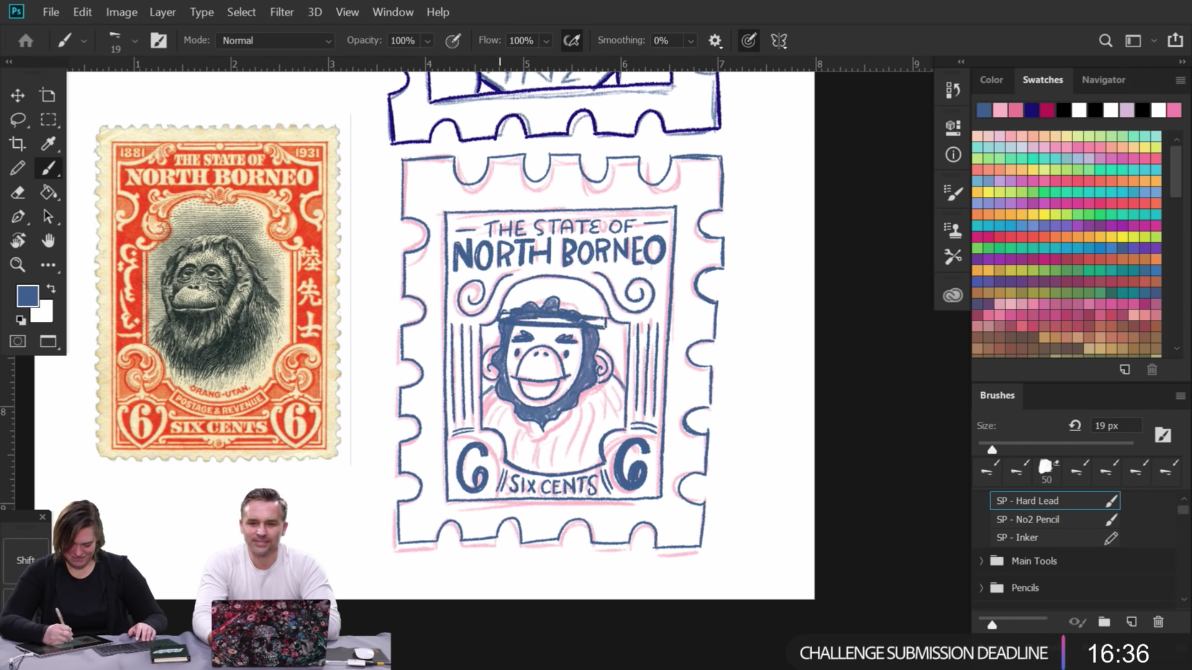
\includegraphics[width=0.6\columnwidth]{liveclips/figures/adobelive.png}
  \caption{The \textit{Adobe Live} series features a guest artist (bottom left) and a host (bottom right). The artist is working on a digital drawing, and the host is looking up at the live chat feed, engaging with the audience (\href{https://youtu.be/yYDmQhg_1uE}{\nolinkurl{youtu.be/yYDmQhg_1uE}}). }~\label{fig:livestream_adobelive}
\end{figure}

\textit{Adobe Live} differs from most streams by featuring two people. Typically there is a host and an guest artist (\autoref{fig:livestream_adobelive}), but sometimes two artists work together. Adobe hosts different artists every week across a range of creative disciplines (\textit{e.g.}, graphic design, UX design, photography, video editing). Typically, the host moderates the stream, responding to chat messages and passing on questions from viewers to the artist so that the artist can focus on their work. When the stream includes two artists, they trade off hosting.
%xxx: removing for now because we haven't talked about challenges for streamers yet
%These live streams address some of the challenges self-streamers often face, such as facilitating the chat while working and dealing with technical setup, by having separate people take on those tasks. 
The featured artists are usually practitioners, not teachers; their work mainly serves as inspirational demonstrations, while also giving the the community a chance to engage with questions and comments. 

The \textit{Daily Creative Challenges} series features one person who both reads chat messages and provides a short tutorial on a software technique. These live streams are part of Adobe's Creative Challenges, which are contests that encourage people to use Adobe software and submit design work for prizes\footnotemark. These streams are 30 minutes long -- this is short for a live stream -- and focus on instruction: explaining the challenge of the day and teaching viewers the skill of the day. 

\footnotetext{\href{https://www.behance.net/dailycreativechallenge}{\nolinkurl{behance.net/dailycreativechallenge}}}

%The interviews and surveys in this paper are with a mix of people from Adobe's live streams and from other creative communities, allowing us to gain a broad understanding of the challenges creative streamers face and suggest possible improvements for them.

\subsection{Why \& How do People Stream Creative Work?}
%Now that we have a broad understanding of two popular creative live streaming communities, we seek to go deeper into the motivations and processes behind creative live streamers. 
What motivates people to live stream creative work? What challenges do they encounter in the process, and how do these compare with streamers in other domains? We interviewed 8 creative streamers and found that streamers were primarily motivated by sharing and engaging with their audience. However, they find it difficult to connect with their audience while focusing on their work. Additionally, for many, live streaming requires significant effort and behind-the-scenes preparation. 

%Streamer motivations and processes seem to be highly dependent on the type of stream they create. Prior work has shown that the main reasons gaming streamers stream are to build a community of like-minded individuals \cite{Hamilton2014, Pellicone2017} and to make money or promote their personal brand \cite{Pellicone2017}. People who live stream about their lifestyle or to entertain do it primarily for personal branding \cite{Tang2016}. In contrast, educational or culture-sharing streamers' main goal is usually to share their knowledge and culture with others \cite{Lu2018a, Lu2019}. As for process, some live streams are highly produced and require significant preparation beforehand (\textit{e.g.}, e-sports tournaments), while others occur on-the-spot whenever the streamer decides to go live (\textit{e.g.}, many lifestyle streams on Instagram).
%Such streamers often care more about making a broad positive impact and raising awareness about their particular activity than making money or receiving gifts from viewers, even when they do also make money as a side benefit \cite{Lu2019}. 
%We echo Lu \textit{et al.}'s \cite{Lu2019} finding (maybe) that for many types of creative activities that are usually solitary (e.g., playing a solo musical instrument or doing visual art), streaming allows people to have company while they work so the activity is not so lonely.

\begin{table*}[t]
\centering
\caption{Self-reported background information about the eight creative streamers we interviewed. ``Skill'' refers to the streamer's skill at the type of creative work they stream. After interviewing the streamers, we determined the structure type of their most frequent streaming style.}~\label{table:livestream_streamers}
\resizebox{1\textwidth}{!}{
\begin{tabular}{llllllll}
            & \textbf{Role}                                                                       & \textbf{Content}       & \textbf{Skill} & \textbf{Frequency} & \textbf{Platform}                                                              & \textbf{Primary type} & \textbf{Moderators} \\
\textit{P1} & Freelance Digital Illustrator                                                       & Digital Illustration   & Expert         & 3 times / week     & Twitch                                                                         & Making                & Yes        \\
\textit{P2} & \begin{tabular}[t]{@{}l@{}}Video Editor \& Educational\\ Content Maker\end{tabular} & Q\&A, Analyzing Videos & Expert         & Occasional         & YouTube, Instagram                                                             & Teaching              & Yes        \\
\textit{P3} & Artist / Musician                                                                   & Music Improvisation    & Expert         & Occasional         & Facebook, Instagram                                                            & Performing            & No         \\
\textit{P4} & Drawing Hobbyist                                                                    & Digital Drawing        & Intermediate   & Monthly            & Twitch                                                                         & Making                & No         \\
\textit{P5} & Drawing Hobbyist                                                                    & Digital Drawing        & Intermediate   & Monthly            & Twitch, previously Picarto                                                     & Making                & No         \\
\textit{P6} & Adobe XD Evangelist                                                                 & UX Design              & Expert         & Daily - Weekly     & \begin{tabular}[t]{@{}l@{}}YouTube, Facebook,\\ previously Twitch\end{tabular} & Teaching/Making       & Yes        \\
\textit{P7} & Adobe XD Evangelist                                                                 & UX \& Graphic Design   & Expert         & 3 times / week     & \begin{tabular}[t]{@{}l@{}}YouTube, Periscope,\\ Facebook\end{tabular}         & Teaching/Making       & Yes        \\
\textit{P8} & Adobe Designer                                                                      & UX \& Graphic Design   & Expert         & Daily - Weekly     & YouTube, previously Twitch                                                     & Teaching/Making       & Yes       
\end{tabular}
}
\end{table*}



\subsubsection{Interview methodology}
We recruited 8 streamers (4 male, 4 female, ages 20-45) from personal and professional connections for one-hour semi-structured interviews. We interviewed people across creative disciplines and experience with streaming (\autoref{table:livestream_streamers}). We asked participants about their current position and background, process and motivation for streaming, challenges and successes they have experienced, and strategies for engaging with their audience. Three of the participants also host for \textit{Adobe Live}; we asked them about their experience hosting as well as streaming. We took notes and recorded every interview, and analyzed them by comparing participants' answers and identifying common patterns. Interviews were conducted over video chat (4), audio chat (2), or in person (2). Each participant received a \$15 gift card for their time. 


\subsubsection{About the streamers}

\textit{P1} is a freelance artist who began streaming her work full-time on Twitch in 2016. For the first two years, she streamed for 20-25 hours a week and spent the rest of her time on stream-related preparation. At this commitment level, streaming was her primary source of income. Income on platforms like Twitch mainly derives from ad revenue, viewer subscriptions, and donations. Over time, this became exhausting and felt unsustainable. \textit{P1} took a break, and now streams casually 3 times a week but not as a primary source of income. Her live stream setup includes a camera view of her face, a screencast of her work, a Stream Deck (\autoref{fig:livestream_streamdeck}), and two monitors for her to see chat activity and other information.

\begin{figure}[b!]
\centering
  
\includegraphics[width=0.5\columnwidth]{liveclips/figures/streamdeck.png}
  \caption{The Stream Deck is a programmable control pad used by many streamers, including \textit{P1}, for easy access to common shortcuts and actions. It integrates with Open Broadcaster Software (OBS), a program used by many streamers to host their live streams (\href{https://www.elgato.com/en/gaming/stream-deck}{\nolinkurl{elgato.com/en/gaming/stream-deck}}).}~\label{fig:livestream_streamdeck}
  \vspace{-0.2in}
\end{figure}

\textit{P2} is a video editor and creator who has been making video tutorials on photo and video editing for about 7 years. He hosts a podcast where he interviews people about their creative approach and life stories. He has tried Periscope, and began streaming on YouTube when it enabled mobile streaming in 2017: casual streaming was on the rise. Occasionally he live streams on YouTube or Instagram, answering viewer questions, teaching a particular topic, analyzing a popular video, or critiquing viewers' work. His setup comprises a camera view of his face, a screencast of his work, and a large monitor for him to see chat activity and other information.

\textit{P3} is a musician who live streams on Facebook and Instagram (with three band members). Her streams are spontaneous and improvisational; the quartet does not play together regularly but they have a fan base that they stream to whenever they are together. These streams require little setup; they are broadcast from a single mobile phone either held by a friend or propped up. She also occasionally streams product reviews and behind-the-scenes views of her shows.

\textit{P4} and \textit{P5} are hobby artists who stream digital drawing about once a month on Twitch. They both started streaming 2 or 3 years ago. \textit{P5} used to stream on Picarto, and moved to Twitch about a month ago because it was easier to use and tends to attract more viewers as a better-known platform. \textit{P5} rarely talks out loud during her streams (only when nobody else is home) and \textit{P4} never does. Instead, they engage with viewers by typing in the chat. Neither shows their face when streaming; their setups include only a screencast of their drawing window. 

\textit{P6}, \textit{P7}, and \textit{P8} stream as part of their jobs at Adobe by hosting artists, streaming their own work, and teaching Adobe products.
%are all employees of Adobe who regularly stream on Adobe's Daily Creative Challenges, and also host on Adobe Live. 
%These participants stream frequently as part of their jobs, and are all highly experienced at the creative work they stream. 
\textit{P6} has been making video tutorials on photo editing for over 10 years. He briefly tried streaming on Twitch but found that his audience did not transfer over to the new platform. He has been streaming with Adobe for approximately 6 months. \textit{P7} taught courses and training programs on design and illustration software for many years. He has been working at Adobe for 9 years, and streaming with Adobe for about 4 years. 
%\textit{P7} was one of the first evangelists involved in Adobe's live streaming efforts, which started on Twitch.
\textit{P8} is a designer and trained illustrator and has been streaming with Adobe for 4 years. Before joining Adobe, she used to occasionally stream her art process on Twitch. By virtue of live streaming professionally, all three participants have fairly sophisticated technology setups, including a camera view of their face in front of a green screen, a screencast of their computer, several displays for them to see chat activity and other information, and sometimes additional cameras (\autoref{fig:livestream_adobelive_setup}). 

\begin{figure}[t!]
\centering
  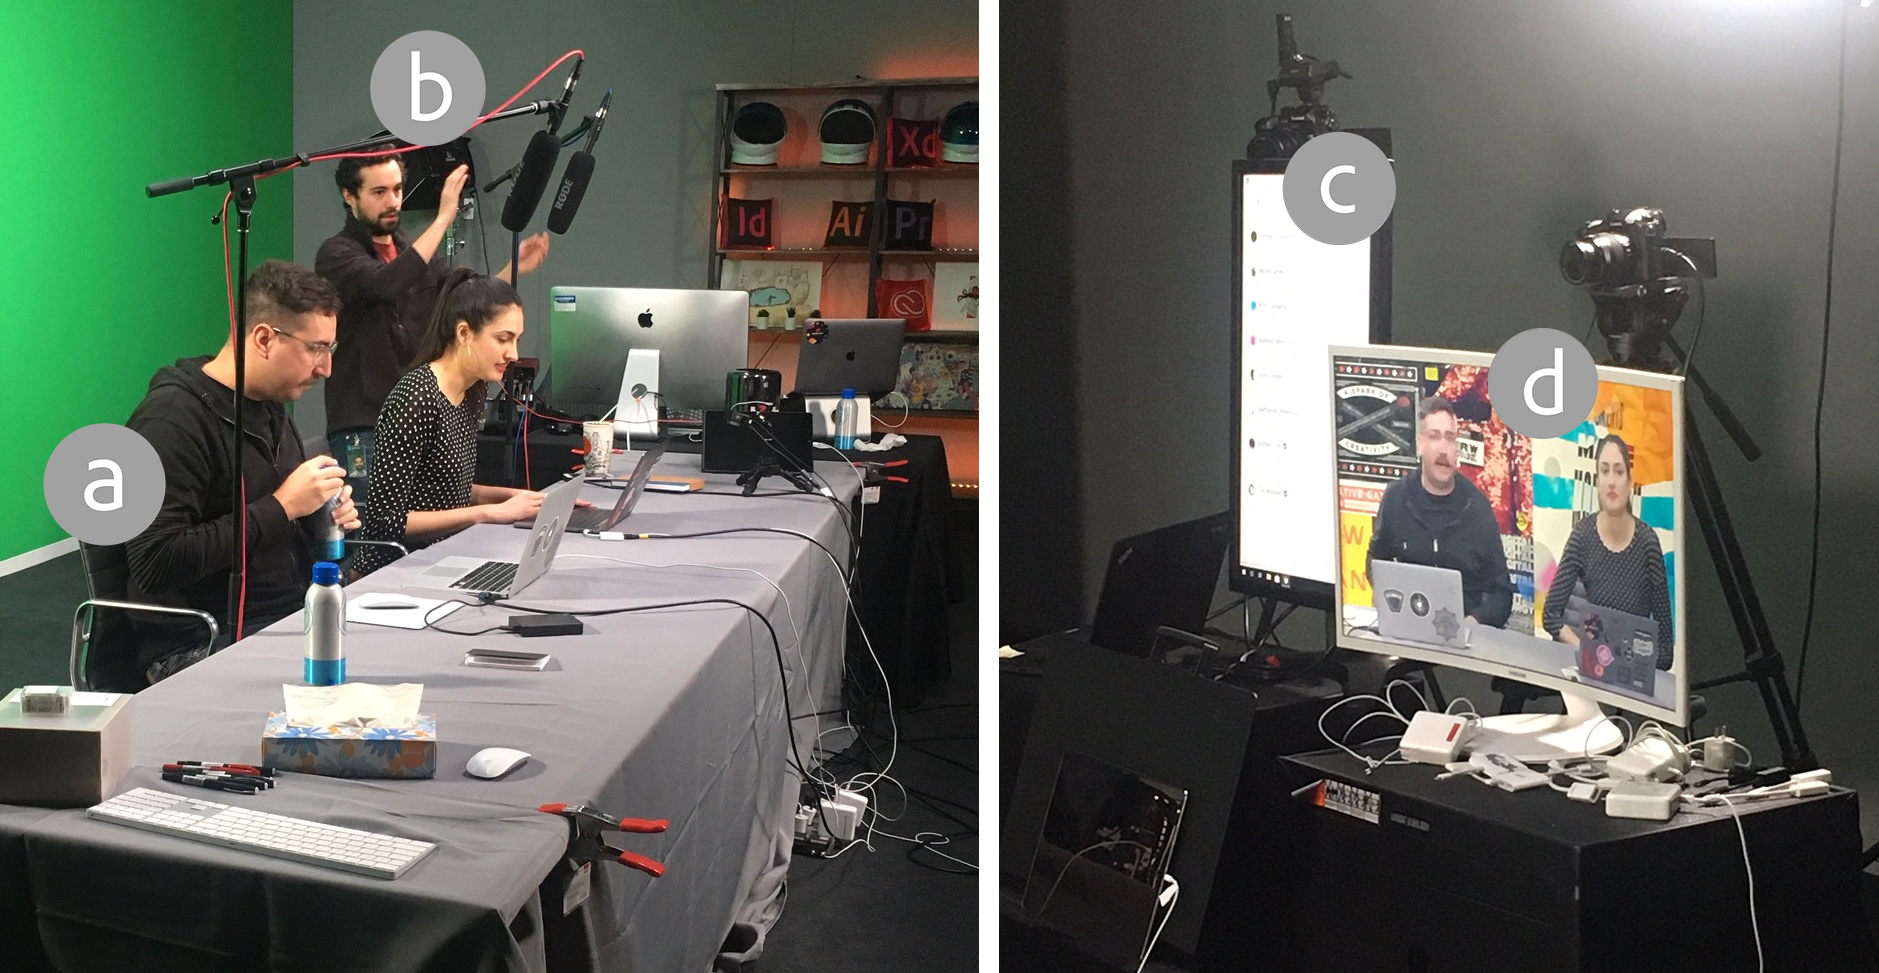
\includegraphics[width=0.8\columnwidth]{liveclips/figures/adobelive_setup.png}
  \caption[The technical setup for \textit{Adobe Live}.]{The technical setup for \textit{Adobe Live}. (a) The artist (left) and host (right) sit in front of a green screen, with both computers connected for screencasting. (b) Behind the scenes, at least one person helps with technical support, including setup, testing, and monitoring. (c) The artist and host see a display with the live chat feed, and (d) a display showing how they currently appear in the live stream. }~\label{fig:livestream_adobelive_setup}
  \vspace{-0.2in}
\end{figure}

\subsubsection{Findings}
\textbf{Audience engagement is a primary goal for streamers:}
Like with gaming \cite{Pellicone2017, Hamilton2014} and culture-sharing \cite{Lu2019} live streams, audience engagement is important to creative streamers. All participants said they engage with their audience during streams, despite their different personalities and streaming styles. When asked about their main motivation for streaming, participants mentioned creating a space for people to hang out together, building an audience, sharing their process with others, and engaging in meaningful conversations.

When asked for an example of a rewarding or enjoyable moment, every participant mentioned audience engagement in some way. Three participants mentioned feeling rewarded by gratitude from viewers for inspiration and community. This inspiration goes both ways: \textit{P5} mentioned that she has received valuable feedback from a viewer that helped improve her own work. Two participants valued that \textit{``there's something more authentic about [live streaming] ... it allows me to just be myself more authentically and people can pick up on that, they can understand what you're really about in a way that you just can't express via [other modalities]''} (\textit{P2}). \textit{``There are really no mistakes, there's just honesty''} (\textit{P3}).

A key difference between gaming and creative live streams affecting engagement is the scale of the audience. The average live audience size for our participants ranged from about 5 to 1000, with most sitting at the lower end. Popular streamers of video games such as Fortnite or League of Legends often average audiences of between 2000 and 40,000. This means that creative streamers often feel a tighter personal connection with their viewers, while viewers of gaming streams tend to mostly interact with each other, as the chat goes too quickly for the streamer to keep up \cite{Lessel2017, Hu2017}.

\textit{P7} expressed a desire to offer the audience more diverse interactive experiences beyond just text chat. Currently, gaming live streams sometimes host ``audience participation games'' \cite{Glickman2018}. \textit{P1} often organizes games during live streams, such as contests with prizes, voting on what she should do next, or ``prompt games'' where viewers contribute ideas. \textit{P4} did a ``request stream'', where he drew whatever viewers requested, and \textit{P2} often runs Q\&A-form streams, where he will open an application and just let the audience ask questions. As he put it, \textit{``I want to do what they want to do.''} \textit{Adobe Live} often has giveaways for audience participation, and Adobe hosts a \textit{Daily Creative Challenge}. This kind of engagement \textit{``make[s] it a collaborative thing''} (\textit{P6}), increasing audience investment.

One emerging practice is live streaming portfolio critiques. Like a call-in radio show or newspaper advice column, a few people get direct feedback, and many people benefit through over-the-shoulder learning. This form of learning can be extremely beneficial \cite{Lopez2010}; it is notable that there is a streaming audience that seeks it out. Similar to shows and columns, streamers have the challenge of selecting which submission(s) to critique. \textit{P2} initially handled this with chat but was quickly overwhelmed by the number of messages. To address this, he found and installed a widget\footnote{\href{https://streamlabs.com/widgets}{\nolinkurl{streamlabs.com/widgets}}} to help him select submissions and allow users to pay a small amount to have their work critiqued. While valuable, it takes time and effort to manage such tools. This also exacerbates streaming's already ``fragmented technology ecosystem'' \cite{Lu2019}.

Aside from the three Adobe participants who stream as part of their jobs, none of the participants currently stream as a major income source. Though these participants were not \textit{primarily} motivated by monetary gain, two mentioned that it was a significant secondary benefit, \textit{e.g.}, \textit{P4} said, \textit{``it doesn't matter how good my work gets if I don't actually market myself.''} Many streamers in other domains (especially video games) also aim to grow their audience and make money \cite{Pellicone2017}. \textit{P1}'s sought to eventually be a self-sustaining artist; she emphasized that her primary goal was building the audience and creating a positive community; \textit{``I believe that the audience brings [financial benefits].''} \textit{P3} wished it was easier for viewers to donate. Compensation is possible on some platforms (\textit{e.g.}, Twitch) but requires configuration.

\textbf{Moderators \& hosts alleviate common challenges for artists:}
A big part of engaging with the audience is interacting via the chat window with viewers' questions, comments, and feedback. 
%interesting: this is indirect engagement
Most participants said they sometimes have trouble keeping up with the chat as it requires switching focus from their creative work. This split-attention challenge echoes previous findings for programming \cite{Faas2018} and culture-sharing \cite{Lu2019} streams.
%- Paying attention to chat and interacting with audience while working \cite{Faas2018}, especially when work is not on the computer \cite{Lu2019} \\
%-- Messages distracting from work, especially when lots of viewers \cite{Lu2019}
\textit{P5} even said, \textit{``I usually put a warning beforehand that I'm not the most talkative while I'm drawing but I try to check up on the chat as often as I can.''} For \textit{P3} who streams on  a smartphone, it is even harder to pay attention to chat, as it requires stopping her performance and coming up close to the camera.

Moderators are one way to alleviate this challenge for viewers. In large gaming live streams, trolling is common; many streamers have dedicated moderators whose main role is to ban or time-out people posting inappropriate content and enforce a streamer's community guidelines \cite{Seering2017, Lo2018, Seering2019, YvetteWohn2019}. Trolls are seen less often in smaller live streams, yet still appear; 5/8 participants have dedicated moderators. As prior work has shown  \cite{Lo2018, Seering2019, YvetteWohn2019}, employing successful moderators requires significant preparation; streamers must work with moderators to develop guidelines, and they must constantly work to make sure their judgments align. \textit{P1} and \textit{P2} echoed these challenges: \textit{P1} has spent significant time making a document of guidelines for her moderators. \textit{P2} has not, and as a result finds that their judgments do not always align: \textit{``They might want to ban someone that I think is fine, or they might not ban someone that I think should be banned.''}

While moderators can help enforce basic rules and keep the chat constructive, they usually do not support streamers' \textit{engagement} with their audience. Viewers often have questions, feedback, and suggestions for the streamer; these are easily missed. Some moderators do engage in the chat \cite{YvetteWohn2019} but they require training in order to answer questions on behalf of the streamer (\textit{e.g.}, \textit{P1}'s moderators). In addition, some streamers find it difficult to talk out loud to their viewers: both \textit{P4} and \textit{P5} said they would like to have others to talk with, as they did not want to fill the silence alone; \textit{``I'm mostly intimidated by the idea of me having to fill a lot of void space''} (\textit{P4}). While \textit{P4} used Discord and \textit{P5} sometimes used join.me for voice chat, these require extra work on the part of the streamer, and sit outside of the main live stream platform.

A different facilitation role that Adobe streams employ to address these challenges are \textit{hosts}. \textit{Adobe Live} streams feature paid hosts who keep the artist and audience engaged, help artists feel confident, and help them focus on their work. The host watches chat messages come in, says hi and responds out loud to viewers' messages, and decides which of viewers' questions to ask to the artist. As \textit{P7} put it, the host is the \textit{``representative for the chat.''} Hosts strive to keep viewers engaged by asking the chat questions and including viewers' names when they respond to them. Hosts also strive to keep the \textit{artist} engaged and talking. As \textit{P6} put it, \textit{``the last thing you want is dead silence.''} This can be difficult when the artist is shy or quiet, so hosts have picked up tricks such as asking the artist questions about themselves, choosing questions from the chat that are likely to start a conversation, and switching the feed briefly over to their computer to show a relevant tip or trick.


%xxx: commenting out for now
%- moderators can be co-present or telepresent
%- some streamers sometimes have co-present people (helping, audience, etc)

\textbf{Different platforms bring different audiences:}
Some participants stream on multiple platforms. Some start streaming on one platform and then switch to another. This brought up interesting trade-offs between different types of live streaming platforms. Besides mobile platforms being simpler than desktop, different platforms also bring different audiences. \textit{P6} and \textit{P8} used to stream on Twitch before Adobe's live streaming community started. They explained that Twitch is a general-purpose platform dedicated to live streaming. It attracts people who generally enjoy live streams and may be interested in creative work but are less often professional. On Twitch it's harder to attract people who are less familiar with live streams, perhaps because of unique specific features such as ``emotes''; as \textit{P1} explained, \textit{``if you are in the ecosystem you're really happy with it, and if you're not in the ecosystem it's bizarre.''}

\textit{Adobe Live} is an example of a professionally-managed live\-stream aimed at a company's customers. As a result, it tends to attract aspiring designers and creatives who use the software being shown and want to learn how to produce better work. It also attracts more people who are not familiar with live streaming, as it is shown on platforms that also include other forms of media (Behance and YouTube). A challenge with platforms like this is that \textit{``people might not really get ... why watch a live stream''} (\textit{P2}), as it is not yet widely understood.

Finally, platforms like Picarto focus specifically on \textit{creative} live streaming. These attract viewers dedicated to the topic, which can make conversations more focused. The challenge with specific platforms like these (at least in an era where the phenomenon is still growing) is that fewer people have heard of them, so it can be harder to attract viewers. For this reason, \textit{P5} switched to Twitch. Indeed, Picarto generally has 100-200 streams live at any given time, which is considerably less than the Art section alone on Twitch (which has over 300).

The type of creative work being done also affects the audience. For participants who do visual art such as drawing or use creative software, their streams tend to be of the Making or Teaching type, and their audiences mainly comprise other artists or people interested in learning the skill. For \textit{P3} who streams Performing content on Facebook, her audience mainly consists of friends and fans. These viewers enjoy watching the performance and being a part of live music, but are not necessarily looking to learn music themselves.
 
%\subsection{Streaming often requires setup and preparation}
\textbf{Amount of preparation depends on stream type \& preferences:}
While gaming live streamers can simply turn on their screencast and begin playing a game, creative streaming often requires more preparation. 6/8 participants said they prepare before beginning a live stream. Four of these primarily run Teaching streams; the other two primarily run Making streams. For Teaching streams (\textit{P2}, \textit{P6}, \textit{P7}, and \textit{P8}), the streamers spend time before the stream going over what they will show. For Making streams, \textit{P1} and \textit{P5} spend time on the early stages of their creative work. In addition to preparing content, live streaming (especially on desktop platforms) also requires technical setup. Most participants who stream on desktop platforms said this takes time: setting up cameras and microphones, organizing windows across multiple displays, and testing the output.

Most Teaching streams require some content preparation, much like how course instructors make lesson plans. Socializing streams likely require little-to-no preparation, as the content of these streams is mainly driven by conversation with viewers. For example, \textit{P2} sometimes streams casual Q\&A streams on Instagram, enjoying their spontaneous nature: \textit{``you just go live.''} For Making and Performing, preparation time depends on the streamer. Some streamers also announce beforehand when they will stream so that viewers can plan to tune in.
%i said it better. but dont remember how
For casual Performing streams like \textit{P3}'s, all she has to do is turn on the camera and position it. But rehearsed performances require practice beforehand. \textit{P4} said he typically only plans his Making streams 5 minutes before starting, and will start drawing from scratch on the stream. \textit{P8}, who used to do more Making streams, also did not prepare: \textit{``it's as if I am opening up my sketchbook and my friends are there.''} Other Making streamers like \textit{P1} and \textit{P5} prefer to start their work before beginning a stream.

Several participants emphasized that some activities make for more engaging live streams than others. Both \textit{P1} and \textit{P5} said their streams are most successful when they do initial sketching beforehand, then spend the stream filling it in and coloring. This is because the early ideation stages involve more problem-solving and deep thinking: \textit{``to be able to put that full energy ... to get through the failures and to find the successes -- I can't multitask it.''} \textit{P5} also felt this early stage was less appealing for audiences: \textit{``For a long while they're going to have to look at a blank sheet of white `paper' so they don't really see the sketches right away ... I think that loses their attention.''} \textit{P2}, when asked why he doesn't live stream his video editing process, he said he tried it but it was too difficult to focus: \textit{``when you're video editing you need to listen to music and focus ... when you're streaming you need to be engaging with the chat.''} This echoes previous findings for knowledge-sharing \cite{Lu2018a} and programming \cite{Faas2018} streams; streamers often prepare beforehand to ensure that the content being streamed will be entertaining for viewers and will not require too much focus on the streamer's part. 

% other challenges:
% -- Delay between video and chat \cite{Lessel2017} \\
% - Entertaining both novice and expert viewers \cite{Faas2018}
% - fragmented technology ecosystem, hard to manage everything \cite{Lu2019}
% - narrating while also focusing on work \cite{Faas2018} \\
% -- Balancing entertainment with showing realistic process \cite{Faas2018} \\

\textbf{Permanence of live stream archives affects performance:}
We found that the ability to archive live streams significantly affects how streamers perform. Several interviewees mentioned that attentiveness to viewers of a future recording influenced their choices in the moment. \textit{P7} said he sometimes records learning-focused live streams that are meant to be useful as replays, and he interacts less with viewers during those streams. \textit{P2} often deletes or hides his completed live streams because they look less polished than his regular tutorial videos. 
\textit{P4} and \textit{P5} don't archive their videos, as \textit{``[live streaming is] more of a in-the-moment [thing]''} (\textit{P5}). 



\subsection{Why do People Watch Creative Live Streams?}
Every live stream needs an audience. To understand the motivations and challenges of viewers, we conducted three surveys over 1.5 years with 165 people: two with \textit{Adobe Live} viewers; one with viewers of any creative live streams on the Web. All three surveys were voluntary. We found that creative live stream viewers watch streams primarily for \textit{learning} and \textit{inspiration}; community engagement and entertainment were also popular reasons for watching streams. Compared with prior work on live stream viewers in other domains, inspiration is a much more prominent theme in these survey responses.
%In particular, the unique combination of learning with entertainment and engagement that live streams offer makes them an appealing choice over other types of learning-focused content.

\subsubsection{Survey methodology}
The first survey with \textit{Adobe Live} viewers (\textit{S1}) was posted periodically in the chat and overlaid on the stream for four months (August - December 2017). It asked about viewers' experience with creative software, the reasons they watch creative live streams, what other creative live streams they watch besides \textit{Adobe Live}, and how \textit{Adobe Live} streams could be improved. 98 people completed this survey.

A year later, \textit{Adobe Live} had changed considerably: more frequent streams, more audience interaction, and wider and more regular marketing. In January 2019, we conducted \textit{S2} to gain additional insights about viewer motivations and challenges, focusing especially on the live chat experience. The survey was sent directly to previous winners of Adobe's \textit{Daily Creative Challenges} who also showed up regularly in past chat logs of Adobe streams. 41 people completed this survey.

Finally, to zoom out and capture a broader range of creative live stream viewers, we conducted a third survey (\textit{S3}) with viewers of creative live streams on \textit{any}  platform. The survey was disseminated with a snowball method, via the researchers' personal social media accounts. Participants were required to have viewed creative live streams before, which were defined as ``activities such as visual art (drawing, painting, etc.), crafts, music performance, cooking, DIY projects, programming, etc.'' This survey asked viewers about the streams they watch, motivations for watching them, examples of things they learned from them, what else they do while watching, and on which platforms they watch. 26 people completed this survey.

\begin{table}[t]
\centering
\caption{All platforms listed more than once in at least one survey by respondents when asked where they watch creative live streams.}~\label{table:livestream_platforms}
\begin{tabular}{lcccc}
          & \textbf{\begin{tabular}[c]{@{}c@{}}Survey 1\\ $n=98$\end{tabular}} & \textbf{\begin{tabular}[c]{@{}c@{}}Survey 2\\ $n=41$\end{tabular}} & \textbf{\begin{tabular}[c]{@{}c@{}}Survey 3\\ $n=26$\end{tabular}} & \textbf{\begin{tabular}[c]{@{}c@{}}Total\\ $n=165$\end{tabular}} \\
YouTube   & 40                                                                 & 17                                                                 & 17                                                                 & 74                                                               \\
Twitch    & 9                                                                  & 4                                                                  & 17                                                                 & 30                                                               \\
Facebook  & 5                                                                  & 4                                                                  & 4                                                                  & 13                                                               \\
Periscope & 1                                                                  & 1                                                                  & 2                                                                  & 4                                                                \\
Instagram & -                                                                  & -                                                                  & 6                                                                  & 6                                                                \\
Phlearn   & 2                                                                  & -                                                                  & -                                                                  & 2                                                               
\end{tabular}
\end{table}

\subsubsection{What do people watch, and where?}
The most popular platform overall was YouTube (74), with Twitch second (30) (\autoref{table:livestream_platforms}). This is likely skewed by the fact that \textit{Adobe Live} is on YouTube. \textit{S3} had a smaller sample size but found YouTube and Twitch to be equally popular.

\textit{S3} respondents listed content genres they frequently watch live. Categories that came up more than once were programming (11/26), cooking (6/26), digital art (\emph{i.e.}, digital painting, photo editing) (5/26), music (4/26), physical artwork (i.e. drawing, painting) (3/26), 3D modeling (2/26), and DIY (2/26).

\subsubsection{Viewers watch for learning and inspiration}
Viewers responded similarly about motivations in all three surveys. Despite the differences in sample sizes and populations, this suggests that \textit{Adobe Live} viewers' responses may often align with viewers more broadly. Across all three surveys, learning was the most common reason people chose for watching creative live streams (\autoref{fig:livestream_survey_responses}). While learning has also been found to be an important goal for viewers in other domains such as gaming, the primary goal most often cited in prior work is entertainment \cite{Lu2019, Wohn2018, Lu2018a, Hilvert-Bruce2018, Faas2018, Cheung2011}.
%In culture-sharing live streams people learn creative skills or techniques \cite{Lu2019}. 
This difference may be due to the prevalence of Teaching live streams in creative communities.

\begin{figure}[b!]
\centering
  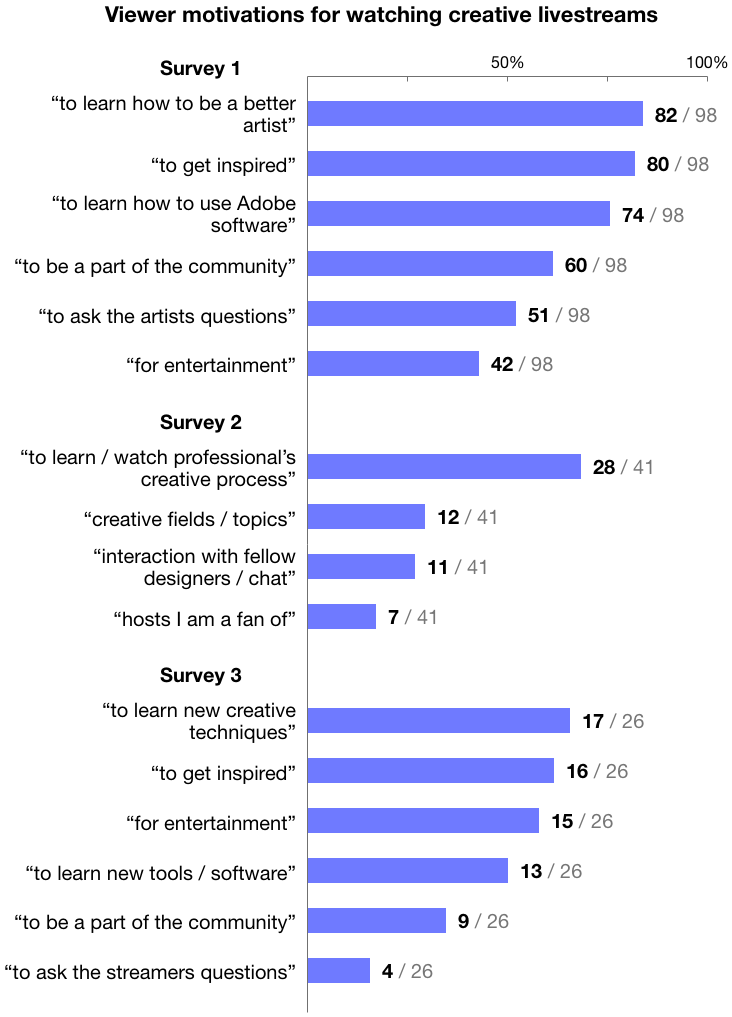
\includegraphics[width=0.7\columnwidth]{liveclips/figures/survey_responses.png}
  \caption{All three surveys asked why people watch creative live streams, allowing them to select all answers that applied from a list. This figure shows all responses chosen by at least 15\% of respondents in each survey. }~\label{fig:livestream_survey_responses}
\vspace{-0.15in}
\end{figure}

Almost all free-form elaborations on viewer motivation mentioned learning. Unlike tutorials and lecture videos, live streams offer direct interaction with the streamer and other viewers, improving the learning experience \cite{Lu2019, Faas2018}. In this way they go beyond just learning content and catalyze ``mentorship communities'' of people with similar interests \cite{Faas2018}. Learners can follow along like an apprentice in a studio, asking questions in the moment. This ability to see authentic, worked examples from start to finish reveals how the streamer makes decisions and recovers from errors \cite{Faas2018}. Viewers often use the knowledge and techniques they learn from creative live streams to inform their own work, as many \textit{S1} respondents stated in free-form responses. \textit{S3} asked for specific examples; 50\% of respondents provided one. They include adopting new techniques such as photo editing operations, trying out a streamer's creative style for things like musical playing or code commenting, and learning how to achieve a specific goal like fixing a hole in a sweater.


In addition to learning, many also reported watching for inspiration / motivation. With one exception \cite{Cheung2011}, primary work has not reported inspiration as a goal. Cheung \& Huang \cite{Cheung2011} describe ``the Inspired'' as one of nine personas for gaming live stream viewers; watching someone stream the game inspires them to play it themselves. However, a large majority of gaming stream viewers watch for entertainment, learning, or providing commentary. While inspiration can be beneficial in many genres, we believe it is especially salient in creative live streams due to inspiration's value for creative work \cite{Herring2009}.

In both \textit{S1} and \textit{S3}, inspiration was the second most popular motivation for watching creative live streams. In addition, 27\% (26/98) of \textit{S1} respondents specifically mentioned inspiration or motivation in free-form responses. 10\% (10/98) also mentioned that the videos helped increase their own motivation and confidence as artists. As one respondent explained, \textit{``[I] like watching artists work because it takes the mystery out of what they do.''} Another said, \textit{``Watching experts make mistakes gives me confidence.''}

Creative work is often a solo activity, and its nebulous nature can make it hard to stay motivated as an artist, often causing creative ``blocks'' such as writer's block. Watching someone else work can motivate viewers to keep going, as well as give them new ideas to try. Respondents in all three surveys mentioned this in free-form responses. For example, one \textit{S1} respondent said they watch live streams for \textit{``getting myself inspired and hyped before I start working.''} An \textit{S3} participant said, \textit{``It's fun seeing someone else's creative process, and usually motivates me to do my own side projects.''}



%In \textit{S2}, 85\% of respondents said they had watched live streams of a creative activity they would not have otherwise been interested in, indicating that live streams can be a good way to discover new topics.

%not directly trying to learn but more get general creative ideas, motivate them to try their own creative projects, and inspire them to see that anyone can do creative things. 


\subsubsection{Viewers also watch for community and entertainment}
People watch all kinds of live streams for entertainment \cite{Wohn2018, Lu2018a, Hilvert-Bruce2018, Faas2018, Cheung2011}. It may be the streamer's personality or style, the chat, or the content itself. %Even though live streams may have long periods of down time with little activity, their unpredictable nature makes them ``engaging but dull'' \cite{Haimson2017}.
People also watch live streams for community. Viewers often feel emotionally attached to the streamer \cite{Wohn2018, Hu2017}, enjoy connecting and conversing with other viewers \cite{Lu2019, Lu2018, Hilvert-Bruce2018}, and enjoy being able to influence the streamer's content or process in real time \cite{Lu2018a}. Live stream communities often lead to longer-term chat groups on other platforms \cite{Lu2018a, Faas2018}.

All three surveys found community and entertainment to be secondary motivations (\autoref{fig:livestream_survey_responses}), showing that these are also important motivators for creative live stream viewers. Several \textit{S1} respondents valued the company of other creative people while they worked alone. To investigate this further, Surveys 2 and 3 asked what people do while watching live streams (multiple choice). 68\% (28/41) of \textit{S2} respondents said they watch while doing creative work. 69\% (18/26) of \textit{S3} respondents said they watch while working on something, and 31\% (8/26) said they work on a similar task as the streamer. In this way, creative live stream communities offer a virtual co-working space for people who would otherwise be working alone.

Respondents in all surveys specifically mentioned that the \textit{combination} of learning and entertainment was what drew them to live streams. This echoes Lu \textit{et al.}'s findings with knowledge-sharing streams \cite{Lu2018a}: they are appealing because they disseminate knowledge in a more relaxed, casual way than tutorials or lecture videos.


%Finally, people watch live streams for community and social engagement. Viewers of a particular stream share a common interest, and the live chat feature of live stream platforms makes it easy for these viewers to connect with each other as well as with the streamer \cite{Hu2017}. 


\subsubsection{What are the challenges for viewers?}
\textit{S1} and \textit{S2} asked how the viewing experience might be improved. The most popular suggestions had to do with interactivity and engagement between the streamers and the chat. 17\% (7/41) of \textit{S2} respondents said their questions often get lost in the chat. Busy chat feeds are a problem in other types of live streams as well \cite{Miller2017}, but can be especially frustrating for viewers seeking to learn and ask questions. Two respondents in \textit{S1} wished that hosts would interact more with the chat, and three others emphasized hosting skill, saying that the best hosts are able to keep the conversation interesting and interact meaningfully with the audience. Two respondents in \textit{S2} wished there were more ways to involve the chat, \textit{e.g.}, through quizzes or polls. Finally, several respondents mentioned that the experience watching replays could be improved; one \textit{S1} respondent said a summary document with important links and tips could help with reviewing the stream later, and three \textit{S2} respondents wished they could view the chat and somehow be involved in the stream when watching replays. This agrees with Lu \textit{et al.}'s findings \cite{Lu2018} that it can be hard to learn from a stream after the fact, as navigation options are usually limited.

\subsection{Summary of Findings}
This section's surveys and interviews uncovered the many goals and motivations streamers and viewers have for creative live\-streams. We also found that existing platforms do not support all these goals or offer help when goals conflict. Specifically, viewers often seek inspiration from creative live streams, but live stream viewing takes place out of context of the viewer's own work. Moreover, despite the wealth of expert knowledge and inspiration such videos contain, watching them as archives is tedious and difficult. Several survey participants mentioned the viewer experience for watching live stream archives is poor because the videos are long, have limited navigation, and include long periods of downtime and conversation with the then-live chat \cite{Lu2018}. Twitch viewers can create ``clips'' and streamers can create ``highlights'' of interesting moments, but they must remember to do so, and such moments can seem out-of-context when viewed on their own.

Motivated by these findings, the remainder of this chapter explores how we might help creative software users benefit from the wealth of expert knowledge hidden in creative live streams without having to watch all the downtime and unrelated conversation that comes with it. We do this by capturing the moments of insight and inspiration from creative live streams and bringing these moments into the context of creative software users' workflows.
\section{Design Space for In-Application Video Examples}
\label{sec:liveclips_designspace}
To help inform our decisions in developing LiveClips and explore how users might interact with such a system during their creative workflow, we outlined a design space for systems that present contextual video examples (\autoref{fig:liveclips_designspace}). This design space is informed by our formative findings as well as prior work on contextual assistance in software. The following three sections present the LiveClips system, which includes three alternative interfaces that explore three different points in this space. This section also highlights where RePlay and ReMap (Chapters \ref{chapter:replay}-\ref{chapter:remap}) fit in the design space as compared to LiveClips. Most notably, LiveClips differs from RePlay and ReMap in that it presents inspirational content rather than educational, and it presents short tool-focused clips rather than entire task-focused videos.

\begin{figure}[b!]
\centering
  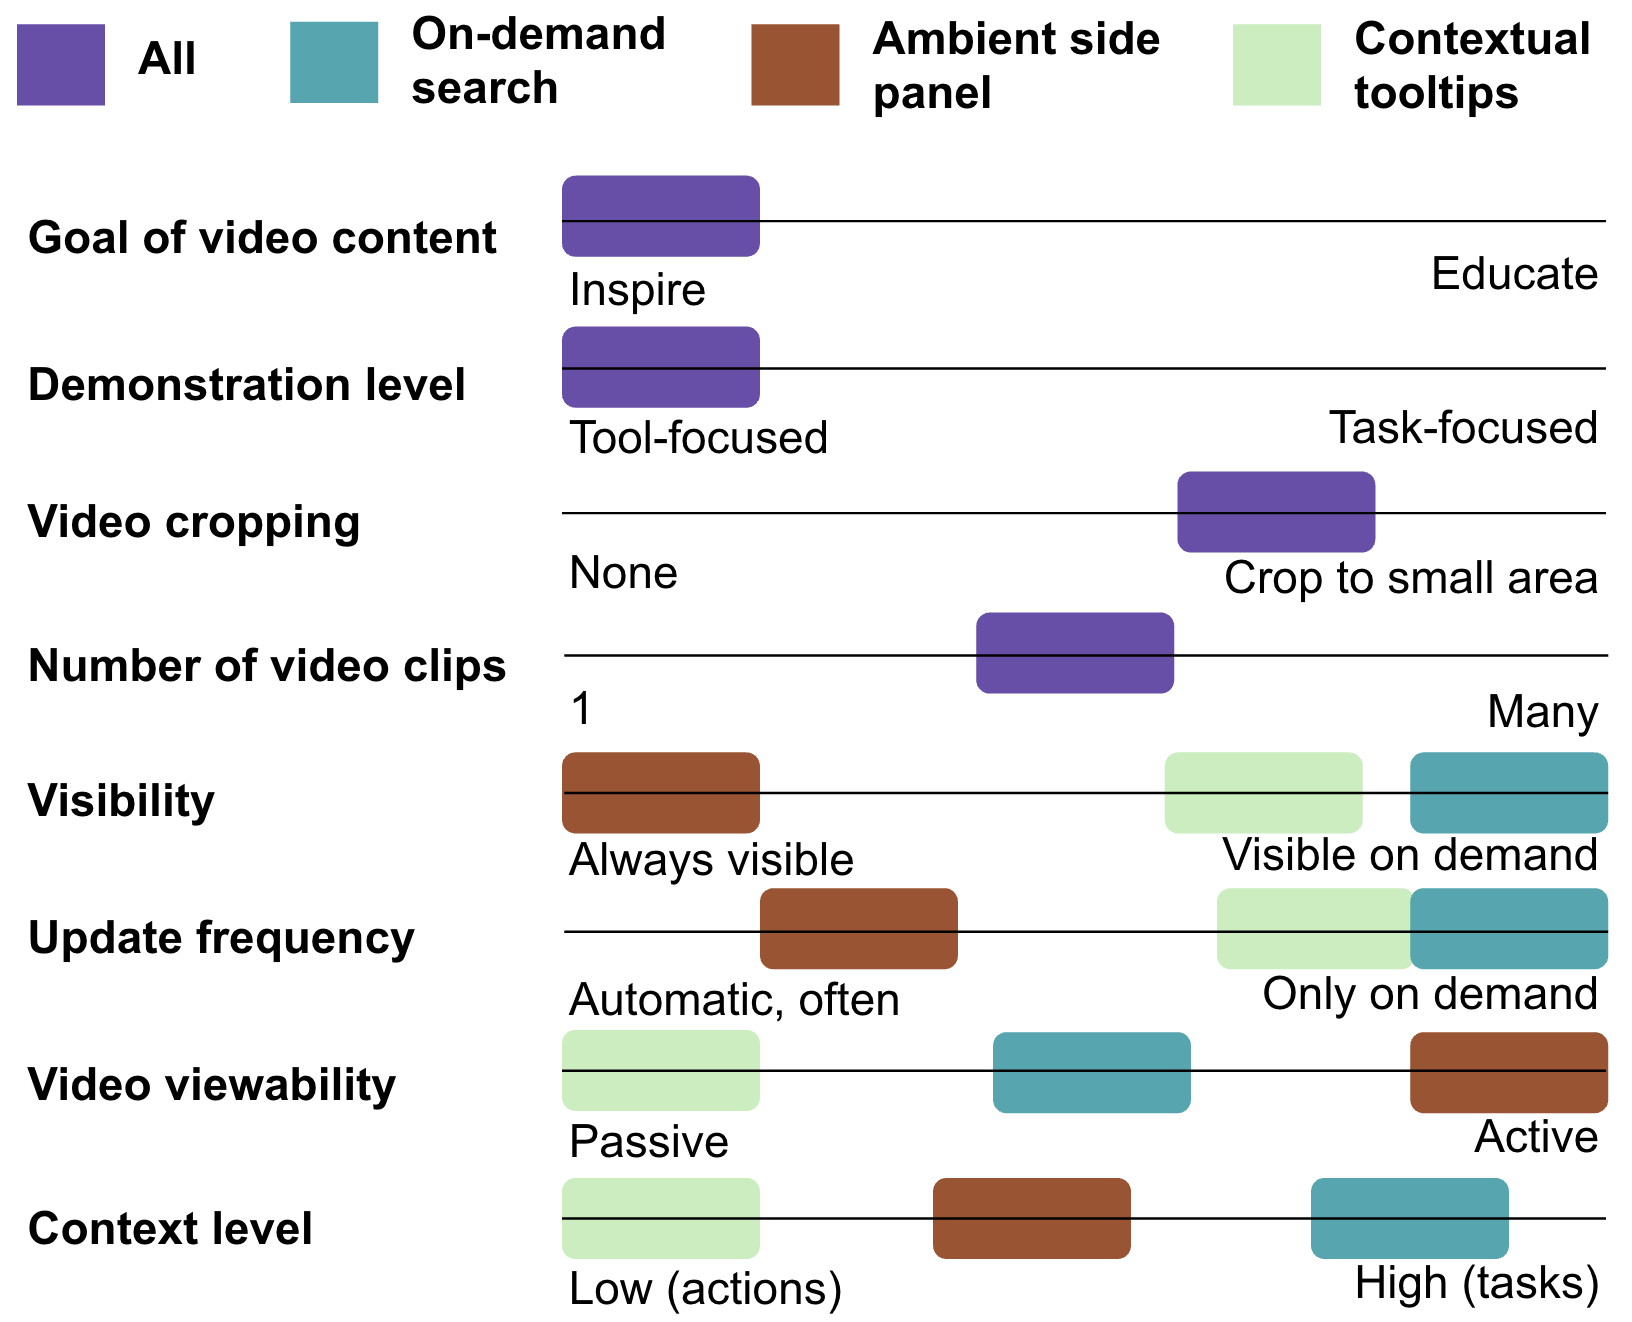
\includegraphics[width=\columnwidth]{liveclips/figures/designspace.png}
  \caption{The design space for in-application video examples, as well as where LiveClips and RePlay/ReMap fit along each axis. LiveClips' prototype interfaces vary along the bottom four axes. }~\label{fig:liveclips_designspace}
\end{figure}

\subsection{Goal of Video Content}
Most prior work regarding contextual videos, including RePlay and ReMap, has focused on content that aims to educate the user, such as tutorials \cite{Pongnumkul2011} and helpful tips \cite{Grossman2010a}. Inspired by the known benefits of examples for inspiration \cite{Kulkarni2014} and our survey findings suggesting that live streamed videos are used for inspiration, this work explores how contextual live streamed videos might inspire users. These videos also have educational value, but this work focuses on them as a source of inspiration.

\subsection{Demonstration Level}
Videos of software use can be tool-focused or task-focused. A tool-focused video demonstrates using a single tool, while a task-focused video shows an entire task from beginning to end.  Tool-focused videos are useful for quick contextual help that does not take away from the user's current work, for example reminding the user how a tool works \cite{Grossman2010a} or showing alternative uses for a tool.
Task-focused videos tend to be longer and are less useful in-the-moment, as they show a specific task that may or may not be relevant. Live streams tend to be task-focused, as they usually follow an artist through an entire task; this work focuses on extracting shorter, more generalizable tool-focused examples from task-focused live streams. RePlay and ReMap also extract relevant moments from within longer task-focused videos, but unlike LiveClips, they are meant for users who proactively seek help with a particular task, so they allow the user to browse the entire video and follow along with it.

%The likelihood that this task will be directly relevant to the user is low \cite{?}. 
%In this work, we focus on creating short tool-focused clips out of longer task-focused videos based on the assumption that shorter bite-sized clips are more useful as in-context recommendation, as they do not take the user away from their current work like a long task-focused clip would. 
%In addition, videos of artists using software often highlight alternative uses for tools that viewers may not have seen before, and so seeing a variety of ways a tool can be used may provide both inspirational and educational value. 

%Many of today's popular creative software applications support a wide variety of workflows. As a result, many of their tools can be used for multiple different purposes and in different contexts. Even expert software users may not be aware of all the different ways a tool can be used. Thus we expect that in addition to providing inspiration, tool-based clip recommendations may help increase users' awareness of the different ways tools can be used. By narrowing in on a focused aspect of a video, we also provide this content in a way that does not detract too much from the task at hand, unless the user wants to see more.

\subsection{Video Cropping}
In-application examples are constrained by space; if content takes up too much space it becomes obtrusive, for example by blocking the canvas where the user is currently working. Therefore, contextual videos must be displayed at a relatively small size. For videos that were created using full-screen video capture (as most live streams are), this can be problematic. Leaving a video un-cropped allows the user to see the full context of interaction but makes it difficult to discern any detail. Since RePlay and ReMap left videos un-cropped, they allowed users to open a single video in a larger window when seeing more detail was necessary. While this may have been practical for task-focused learning where users have other cues to indicate a video's relevance before selecting one (\textit{e.g.}, caption previews), LiveClips aims to show users many examples at once of tool use that may only take place in a small part of the screen. Prior work has explored how to best present video demonstration clips when they cannot be viewed in full screen, by cropping or enlarging sections in the video where mouse movement and canvas changes occur \cite{Chi2012}. Inspired by this, LiveClips crops videos to the area that shows the most visual change, in an effort to make examples focused and easy to browse.

\subsection{Number of Video Clips Shown}
Examples could be displayed one at a time, taking up the least amount of space but also providing less variety. Alternatively, displaying many videos gives users more options but potentially overwhelms them. Prior research on contextual videos recommends displaying multiple videos to demonstrate the range of uses for a tool and increase the likelihood that the user will find at least one useful \cite{Lafreniere2014, Matejka2011}. Similar to RePlay and ReMap (which displayed five videos at a time), our prototypes display four videos at a time in an effort to provide some variety without overwhelming the user or taking up too much space.

\subsection{Visibility}
Examples can be always visible while the user is working (like with RePlay and ReMap), or visible only on demand. Examples that are always visible are more likely to be seen but can be distracting, while examples that are not easily visible and shown only on request are more likely to be ignored or missed \cite{Rhodes1996}. Different users may have different preferences for how visible they want their examples to be, just as some viewers like to watch creative live streams while they work, while others may not. Our prototypes explore three variations along this axis.

\subsection{Update Frequency}
Recommended examples can update in response to an explicit user action (\textit{e.g.}, a query), an implicit user action (\textit{e.g.}, being idle for some time or opening a new document), or automatically at a regular time interval. Updating in response to explicit user actions was appropriate for RePlay and Remap, which are intended to be used when users have a specific question. But for a system like LiveClips that aims to elicit inspiration, the ideal approach is less clear. The trade-offs between these strategies have been widely explored in the literature, and it seems there is no globally optimal solution \cite{Rhodes1996, Chan2017, Siangliulue2015}. Automatic updates can be useful because they require zero effort from the user and can highlight an example in the moment \cite{Rhodes1996}, but they can also distract the user during periods of focused work \cite{Chan2017} or make the interface feel uncontrollable \cite{ODonovan2015}. Updates in response to an explicit request are less distracting and give the user more control over their attention but rely on the user to know when an update would be useful \cite{Rhodes1996, Siangliulue2015}. Update frequency is also tied to Visibility; recommendations that are only visible on-demand only update (visibly) when the user requests them. As with Visibility, the ideal solution may depend on the user's preferences; our prototypes explore three variations.

\subsection{Video Viewability}
When presenting non-static content such as videos in-app, the way in which the user interacts with and views the content may affect its usefulness. On the passive end, videos could play automatically when the content appears, which removes the need for the user to decide whether or not to watch a video but runs the risk of being distracting. On the other end, videos could be shown as a static thumbnail that only animates when the user intentionally interacts. Most prior work  \cite{Grossman2010a, Chi2012}, including RePlay and ReMap, has adopted the latter approach, however such work also suggests that in-context content should have a low threshold for engagement; the user shouldn't have to break too much from their task to interact with recommended content \cite{Grossman2010a}. LiveClips explores three variations along this axis.

\subsection{Context Level}
Examples can vary in how contextual they are to the user's behaviour. Low-level examples respond to the user's individual actions, such as the tools they use. High-level examples respond to the user's task or intent, which can be inferred from sequences of commands or by analyzing the document being edited. RePlay and ReMap use low-level context to augment queries, but the queries themselves can be either low- or high-level depending on the user. LiveClips mostly focuses on lower-level examples, but one of our three prototypes explores a potential way to measure task-level similarity between the user's actions and the examples clip's source video.
\section{LiveClips System Overview}

LiveClips takes as input a live streamed video and telemetry data for the software usage in the video. It extracts short clips showing bite-sized chunks of the artistic process, crops clips to thumbnail size, and ranks clips for recommendation based on their properties as well as the user's context. In the current implementation, audio is removed to focus solely on the visual component of the videos. %(SYSTEM DIAGRAM)

Our approach is tool-centric: each clip focuses on one tool and LiveClips recommends clips based on the user's tool use in the application. We focus on tools as a starting point, because prior work has demonstrated that short tool-focused clips can be effective for contextual learning~\cite{Grossman2010a} and creative software tasks are often centered around the use of different tools.

\section{User Interfaces}
Based on the design space outlined above, we present three alternative methods for displaying and recommending the video clips generated by LiveClips in creative software (\autoref{fig:liveclips_photoshop}).
All three methods provide a link to the original video source underneath each clip, so that users can easily access it if desired. Each interface was implemented as a prototype \textsc{html}/Javascript extension to Adobe Photoshop.

\begin{figure}[t!]
\centering
  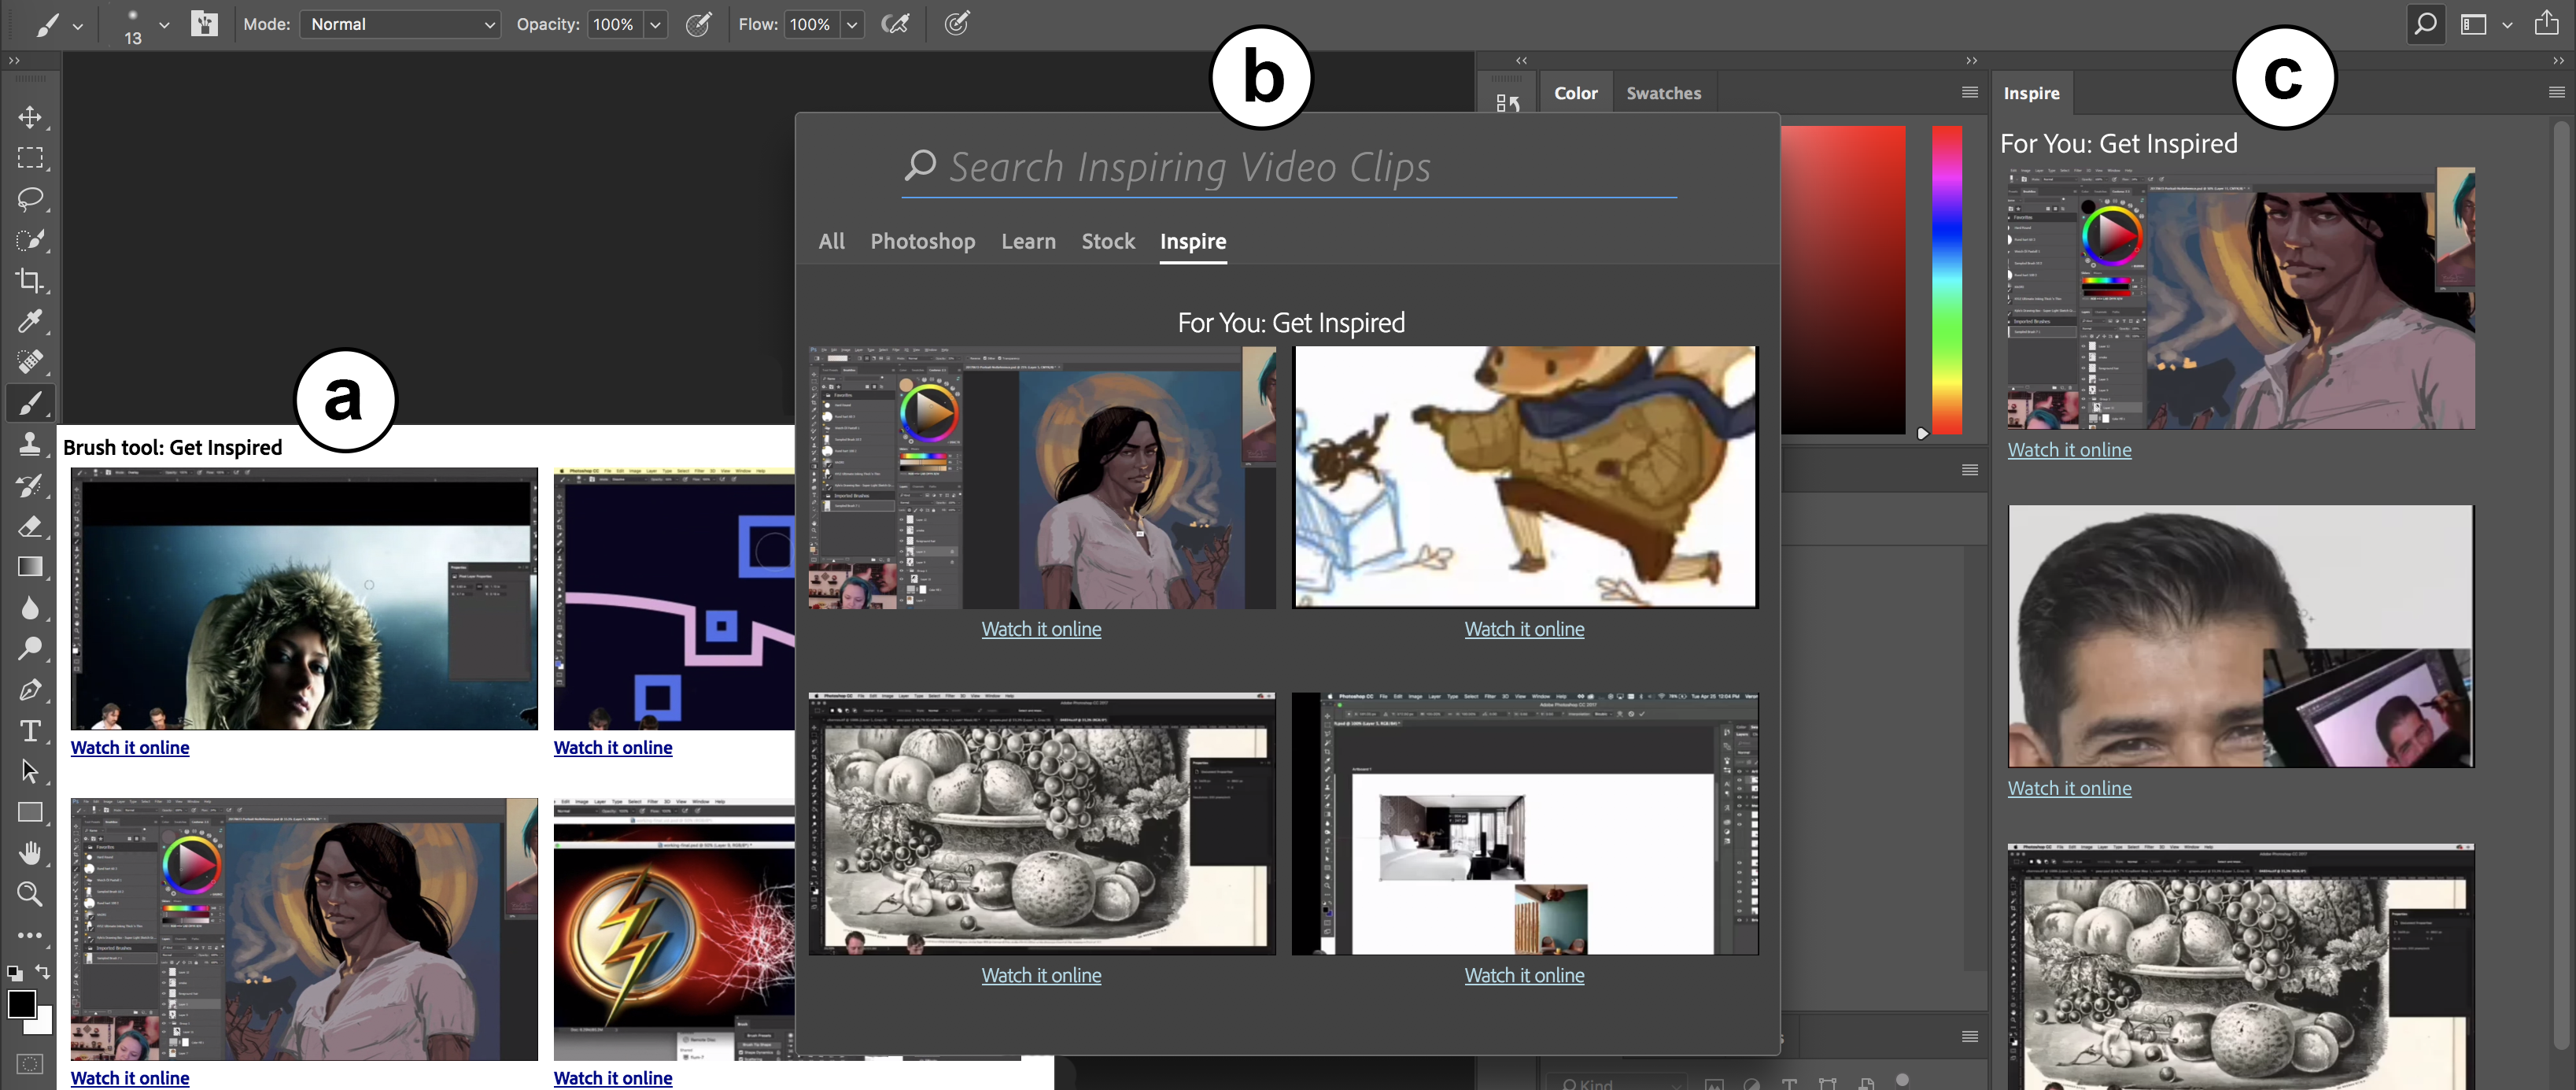
\includegraphics[width=\textwidth]{liveclips/figures/all_interfaces.png}
  \caption[LiveClips' three interface prototypes demonstrate how video clips taken from creative live streams can be embedded in a software tool as inspirational examples, implemented here in Adobe Photoshop.]{LiveClips' three interface prototypes demonstrate how video clips taken from creative live streams can be embedded in a software tool as inspirational examples, implemented here in Adobe Photoshop. a) Contextual tooltips: When hovering over a tool icon, clips of that tool being used are shown. b) On-demand search: Pressing Photoshop's search button or Ctrl-F brings up an extended search interface with task-level clip examples. c) Ambient side panel: an always-visible panel updates periodically with clip examples based on the user's recent tool use. }~\label{fig:liveclips_photoshop}
\end{figure}

\subsection{On-demand Search}
Many software tools provide in-application search, which allows users to search for application features, help, and/or recent documents. We augmented Photoshop's in-application search interface to present four clips when the search window is opened (\autoref{fig:liveclips_photoshop}b). Clips are selected based on the user's tool usage during the entire work session. Users can also search the entire library of video clips from this window. This interface is the closest in concept to RePlay and ReMap's interfaces. As such, we expect this interface to be most useful in moments where the user is stuck and wants new ideas. Each video is displayed as a thumbnail showing the first frame and plays when clicked on.

This interface has low visibility, and updates only in response to an explicit user action. It uses higher-level context to recommend examples. Playback requires intentional mouse clicks.

\subsection{Ambient Side Panel}
Since creative applications tend to include many panels, a natural location for examples is in a side panel. This interface explores examples that update ambiently as the user works (\autoref{fig:liveclips_photoshop}c). To avoid distracting the user during periods of focused work \cite{Chan2017}, the examples only update after the user has been idle for 10 seconds, indicating that they might be taking a break or trying to think of new ideas \cite{Siangliulue2015}. The panel shows four clips based on the user's recent tool use. Mousing over a clip plays it, providing a low threshold for interaction without distracting the user by playing video clips automatically.

This interface has high visibility, updates in response to implicit user actions, and uses mid-level context to recommend examples. Playback requires mouse movement without clicks.

\subsection{Contextual Tooltips}
For an interface that lies between an on-demand window and an always-visible panel, our third approach shows examples in tooltips that appear when the user hovers over a tool icon for 3 seconds (\autoref{fig:liveclips_photoshop}a). Inspired by ToolClips \cite{Grossman2010a}, we believe tooltips may be a useful location for video examples. They can be activated by the user with minimal effort, are easily dismissed, and will not display at all if the user is working quickly or activating tools with keyboard shortcuts.
Tooltips are a natural place for tool-centric examples; the video clips shown are based on the tool selected. Our implementation shows four clips when the user hovers over a tool, and clips play automatically when the tooltip appears.

This interface has mid-level visibility, updates on demand, uses low-level context (tools) to recommend examples, and requires no interaction for video playback. 

\section{LiveClips System for Generating Clips}
The LiveClips system comprises three stages: 1) extracting short 25-second clips based on tool use from long videos, 2) cropping clips so that they can be displayed at thumbnail size, and 3) ranking clips for the three interfaces described above. 

Our approach uses a hybrid of telemetry (recorded usage data) and computer vision to understand and analyze the videos. We note that this could be accomplished entirely with telemetry (as in \cite{Grossman2010, Lafreniere2014}) by instrumenting the artists' software with detailed logging. Conversely, it could be accomplished entirely with computer vision, as prior work has shown that mouse movement and tool selection can be detected from videos alone \cite{Banovic2012, Pongnumkul2011}. In our case (which is not uncommon), we have some usage data that is not fully detailed. Our approach aims to be a catch-all that allows working with a mixed or inconsistent set of data. LiveClips removes all audio from clips during processing, focusing only on the visual component.

\subsection{Available Data}
To develop and test LiveClips, we collected a sample dataset of live streamed videos. In an effort to make the sample as representative as possible, we collected videos from two sources (Twitch and YouTube), from 17 different artists, and for two different software applications: Adobe Photoshop and Illustrator. Videos ranged in length from 30 minutes to 3 hours, giving us a total of 30 hours of video content from 17 different videos. 

For each video we had access to telemetry data at the level of tool usage, which includes time-stamped events for every selection and invocation of a tool (\autoref{fig:liveclips_usage}). Mouse clicks and canvas manipulation details were not available. Our dataset included the use of 36 different tools from the toolbars in Photoshop and Illustrator.  

\begin{figure}[b!]
\centering
  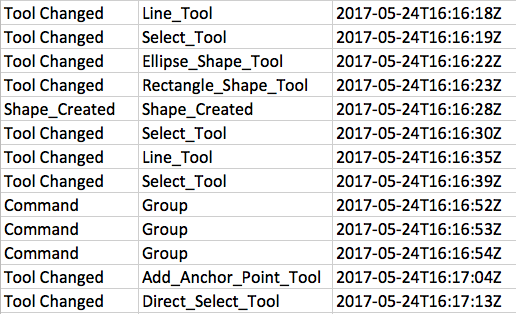
\includegraphics[width=0.5\columnwidth]{liveclips/figures/usage.png}
  \caption{A sample excerpt of the time-stamped usage data we had for each live stream video.}~\label{fig:liveclips_usage}
\end{figure}


\subsection{Extracting Clips}
To extract short clips, we use a heuristic approach based on work by Lafreniere \textit{et al.} \cite{Lafreniere2014}, who segment videos to create instructional clips of tool use. Our focus is on creating inspiring clips, which are different from instructional clips in that they require less attention to specific details (such as setting a tool's parameters) and more attention to the content being created. For the purposes of segmenting initial clips, our method is very similar to Lafreniere \textit{et al.}'s method. We focus on inspirational value in the cropping and ranking stages.

Given a tool, our goal is to create clips showing its use. First, we group all consecutive invocations of the tool and include the tool selection event if it happened within 10 seconds of the first invocation. We add 2 seconds of padding to the beginning so that the viewer can see the tool being selected or invoked. We then trim clips to 25 seconds, as prior work has indicated that 15-25 seconds is a desirable length for in-app video clip recommendations \cite{Lafreniere2014}. We also ignore tool events that are for navigation (\textit{e.g.}, zoom, scroll, select) as these tend to happen frequently in visual software as part of other tasks. We shorten clips where the context likely changed before it was over, i.e. if a document is closed or opened. If a clip is shorter than 15 seconds, we remove it.

This heuristic approach sometimes fails. For example, live streaming artists often work meticulously with one tool for long periods of time (\textit{e.g.}, a brush tool to create artwork), making incremental changes that over time create a more drastic and impressive change. The first 25 seconds of this may not be very inspiring, so we also explore an alternative method for creating clips that brings the focus away from the specifics of a tool's use, and toward the content being created: for instances where a tool is used consecutively for longer than 25 seconds, we extract the entire section where that tool is used, and speed it up to be 25 seconds long. We refer to these as timelapse clips.

In our sample set of 30 hours of video, the above two methods combined produced 1,727 clips, 484 of which were timelapses. This is comparable with Lafreniere \textit{et al.} \cite{Lafreniere2014}, who generated approximately 2500 clips from 25.5 hours of footage. LiveClips generated between 1 and 939 clips for each of the 36 tools in our telemetry dataset.

\subsection{Cropping Clips}
To present examples within an application, they have to be easily viewable by the user. A main design challenge with contextual clip recommendations is the space constraint: prior research has shown that in-app video clips should be unobtrusive and not take up too much of the user's screen \cite{Grossman2010a}. Since live streamed videos typically include the artist's entire screen, simply resizing them to a small thumbnail size will make most of the interesting detail hard to see. Existing methods for cropping videos to a good thumbnail size include cropping it to only the region of the document that changes in the clip \cite{Grossman2010} or cropping to only relevant UI regions \cite{Chi2012}. While more animated effects such as ``pan and zoom'' might be appealing for providing both context and detail, Chi \textit{et al.} \cite{Chi2012} found that too much animation is disorienting for brief video clips.

Since prior work has shown that visible change is an important factor affecting the usefulness of a video clip \cite{Lafreniere2014}, LiveClips attempts to crop each video clip to the area that changes most in the clip, so that the viewer's attention is drawn to the changes that are happening. For inspiration, we are mainly interested in visual change on the canvas. However, there are many other types of visual change that happen in these videos, such as switching windows, opening dialogs, and zooming in and out. Some of these changes (\textit{e.g.}, zooming) are simply uninteresting, and others (\textit{e.g.}, setting parameters in a dialog) may be helpful in a tutorial but are less interesting for short inspirational clips. 
 %The main goal for this content is to expose users to what's possible. Though users might want to see more specifics when they try and follow the artist's method, they will only reach this point if they find the content inspiring in the first place. In such situations, they can click go to the source video and watch the full original video on the Web. 
%
LiveClips therefore excludes these types of change before identifying the area that exhibits the most visual change. This leaves canvas changes and other UI changes. Although we are primarily interested in canvas changes, we leave the task of separating these from UI changes to future work.

To filter out these ``uninspiring'' visual changes, LiveClips uses computer vision to exclude visual change caused by navigational movement, changing application windows, and the artist moving in the webcam view. To detect navigation events, LiveClips does simple feature detection and point feature matching in \textsc{matlab} across consecutive frames to identify and exclude frames where there is a significant amount of motion (likely due to panning or zooming). To detect application window changes, LiveClips identifies moments where more than 90\% of the pixels change between two consecutive frames, and ends the clip before this change occurs. To detect change caused by the artist's webcam view, LiveClips uses face detection in \textsc{matlab} to locate faces that are consistently present in a bottom corner of the screen (which is the customary place for streamers' webcam views) throughout the video, and mask out the corner containing those faces.

To determine the area of most change after filtering out uninspiring changes, LiveClips first calculates the pixel-wise difference between each pair of consecutive frames in the video clip. It then computes the average difference over all of these difference frames. There are many changes around the edges of a clip where artists open menus and panels, but these are not very interesting. The interesting changes are on the canvas, which is typically in the middle of the screen. Thus, LiveClips trims off 100 pixels from all four sides. Next, LiveClips further trims off all sides where the pixel values in the average difference frame are less than a given threshold (which we set to 1/4 of the maximum value in the frame). This allows us to avoid specifying a desired crop size, since some clips may be already zoomed in on the part of the canvas being changed, requiring minimal cropping, whereas others may be zoomed out, requiring substantial cropping to highlight the changing area. \autoref{fig:liveclips_change} shows an example of the average difference frame from a clip and the crop that results from it.
.

\subsection{Ranking Clips for Recommendation}
The set of candidate clips generated is much too large to be useful, as only a few videos will eventually be shown to the user at any given time. As Lafreniere \textit{et al.} \cite{Lafreniere2014} found, over 50\% of automatically selected clips are of poor quality, so choosing good clips from the candidate set is an important step. This section outlines the criteria LiveClips uses to rank clips.

\subsubsection{Time in the original video}
Live streamed videos are several hours long and often show an entire project happening from start to finish. The closer an artist is to the end of their project, the more finished content they are likely to have on their canvas, and thus the more inspiring it is likely to be% (figure showing comparison if time)
. For each clip, LiveClips divides the start time of the clip by the total length of the video to obtain a number between 0 and 1 indicating how far along in the video the clip occurs. Larger numbers are better because they indicate that the clip occurs closer to the end.

\subsubsection{Amount of visual change}
 Lafreniere \textit{et al.} \cite{Lafreniere2014} found that showing clear visual change in short clips was most closely correlated to user preference. To determine how much visual change a given clip shows, LiveClips takes the cropped difference frame generated in the previous stage (\autoref{fig:liveclips_change}), and averages it across the $x$ and $y$ dimensions to obtain a numeric value representing the average amount of change in that clip (a larger number = more change).

\begin{figure}[t!]
\centering
  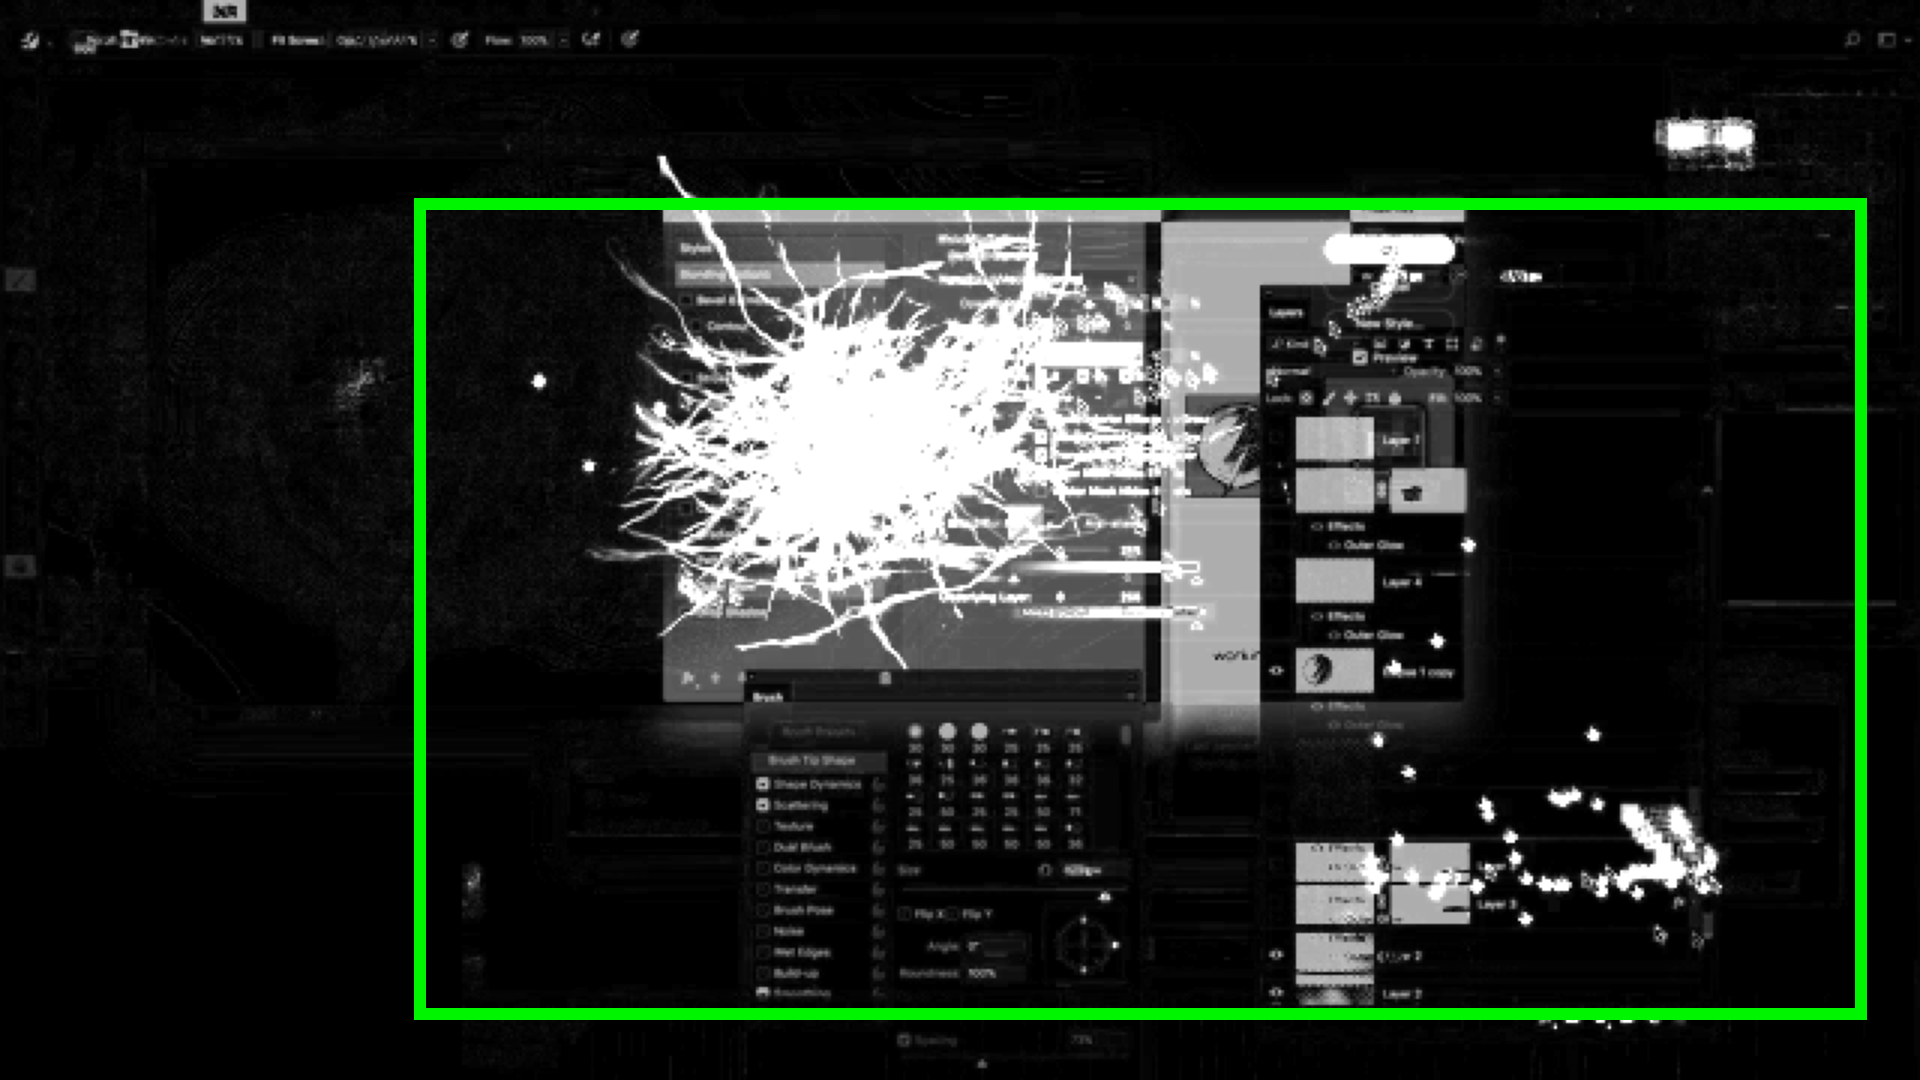
\includegraphics[width=0.7\columnwidth]{liveclips/figures/change.png}
  \caption[An example of a clip's visual change averaged across time (with change caused by navigation, application window switching, and the artist's face moving removed).]{An example of a clip's visual change averaged across time (with change caused by navigation, application window switching, and the artist's face moving removed). From the brightness values of the pixels, we can see that the artist opened some dialogs, and drew some lightning strokes. The green box shows how LiveClips crops the clip to focus on the area that is changing. }~\label{fig:liveclips_change}
\end{figure}

\subsubsection{User context}
User context is the final factor for selecting which video clips to present to the user. This metric varies in each of our three prototypes, to explore different levels of user context. LiveClips' current implementation uses tool use to measure context. LiveClips first calculates a ``total'' score for each clip by normalizing the time and visual change scores from above to be between 0 and 1, then taking the average. (For simplicity, we weight the two metrics evenly.) 

\textbf{Low-level context:} The contextual tooltips interface uses low-level context to recommend examples; video clips are selected based on the tool that the user hovers over. For a given tool, LiveClips orders all clips of that tool by total score, then picks the top four clips. LiveClips requires that all examples come from different source videos, to ensure a variety of content. If some of the top examples are from the same original video, the system goes down the list until it has a set from four different source videos. %In practice, this rarely happens. 

\textbf{Mid-level context:} The ambient side panel uses mid-level context to recommend examples; video clips are selected based on the last four tools the user has used. For each of those tools, LiveClips chooses the clip with the highest total score. If some of these clips are from the same original video, LiveClips instead picks the next top clips that are from different videos, to ensure variety.

\textbf{High-level context:} The on-demand search interface uses high-level context to recommend examples; the user's entire session of tool use is taken into account as well as the entire video from which each clip was extracted. %Many tools can be used for a variety of tasks; for example the brush tool in Photoshop could be used for making a digital painting, or for brushing on a mask to edit a photograph. It is likely that the overall distribution of tools used differs for the above two tasks: a user making a painting would likely spend most of their time using the brush tool and eraser tool, whereas a user editing a photograph might spend some time with the brush tool, and other time with tools such as the clone stamp and the spot removal tool. To recommend videos that more closely match the user's overall task, we therefore look at the time distribution of tool use in each video and compare it with the user's distribution of tool use. 
For each full-length video, we store the overall percent of time spent using each tool, and compare this with the overall percent of time the user has spent using each tool in their current session. To measure the ``difference'' between a video and the user's session, we sum the absolute differences between percentages for each matching tool (each is a number between 0 and 1), and for every tool used in the video that the user has not used at all, we add 1 to the sum. The video with the smallest difference sum therefore represents the closest match to the user's task. LiveClips chooses the live stream videos with the four smallest difference sums. From each video it picks the  clip with the highest total score.% that shows a tool that the user has used in the session.

%To make recommendations LiveClips recommendation engine compares all of the user's recent activity (\textit{e.g.}, which tools are used) to the overall activity in the live stream from which the the clip was extracted. 
%Inspired by CommunityCommands \cite{Li2011}, we consider only usage from the current session, which we define as the time since the user opened the application. For each video, we calculate the percent of time spent using each tool and compare this distribution with the percent of time the current user has spent using each tool. We select the top four videos whose distributions match most closely with the user's, and from each video we select the top ranked clip that shows a tool the user has used. 


%Second method: Recommendations are chosen based on the user's recent tool use, at a lower level than the search interface; every time the the recommendations update, it chooses the top ranked clip for each of the last four tools the user has used.
\begin{figure}[b!]
\centering
  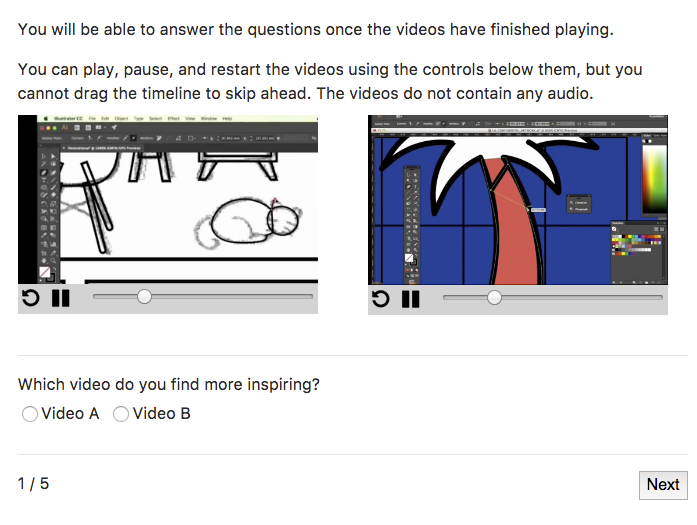
\includegraphics[width=\columnwidth]{liveclips/figures/mturk.png}
  \caption{An example of a pairwise comparison completed by Mechanical Turk workers. Each task involved five such pairs. In the introduction to the task, workers were asked to consider which 25-second video would inspire them to be more creative. }~\label{fig:liveclips_mturk}
\end{figure}

\section{Evaluation}
To evaluate whether our ranking metrics are effective at finding inspiring clips, we conducted a study on Amazon Mechanical Turk. This study did not evaluate clips in the context of creative software. Instead, it focused on whether timing and visual change are good general predictors for inspiring content. 

As described in the System section, RePlay generated 1,742 clips from our dataset of 30 hours of video of Photoshop and Illustrator use. We randomly sampled 129 of these clips to include in our evaluation set. To ensure we had coverage of all tools in our dataset, we randomly chose between 2 and 10 clips per tool. Since some tools are much more popular than others (e.g., Photoshop's brush tool had 939 clips whereas the burn tool only had 2 clips), this method allowed us to have a smaller sample while still representing every tool.

Workers compared video clips in pairs. Each Mechanical Turk task started with an overview page describing the task and showing an example pair of clips followed by five rounds of paired comparisons. Each comparison involved viewing two clips of the same tool and answering which clip they think would inspire them to be more creative (\autoref{fig:liveclips_mturk}). After completing all five comparisons, workers completed a short survey asking about their experience with Photoshop and Illustrator, and what types of creative tasks they do. Workers' results were only included if they completed all of the above steps. In an effort to ensure that they actually watched the videos, each comparison page only allowed workers to answer the question once both videos had played through once. Workers were paid \$1.50 per task, which took an average of 10 minutes and 20 seconds to complete. The same worker could do multiple tasks and would see five new pairs of videos (randomly selected) every time.

\subsection{Results}
In total, 481 workers completed 628 tasks, giving us a total of 3,140 paired comparisons. Most pairs were compared by 9 unique workers, though some ended up being compared more times. To balance results across clips, we considered only the first 9 comparisons for each pair. \autoref{table:experience} shows the distribution of workers' prior experience with Photoshop, Illustrator, and various types of creative tasks. Notably, 73\% and 35\% of participants had at least some experience using Photoshop and Illustrator respectively.

\begin{table}[b!]
\small
\centering
\begin{tabular}{lll}
            &                           & \# Participants \\ \hline
Photoshop   & None                      & 130 (27\%)       \\
experience  & Beginner                  & 242 (50\%)      \\
            & Intermediate              & 91 (19\%)       \\
            & Expert                    & 18 (4\%)        \\ \hline
Illustrator & None                      & 311 (65\%)      \\
experience  & Beginner                  & 114 (24\%)      \\
            & Intermediate              & 46 (9\%)       \\
            & Expert                    & 10 (2\%)        \\ \hline
Creative    & Physical drawing/painting & 247 (51\%)      \\
experience  & Digital drawing/painting  & 147 (31\%)      \\
            & Photography               & 386 (80\%)      \\
            & Photo editing             & 290 (60\%)      \\
            & Design                    & 144 (30\%)     
\end{tabular}
\caption{The distribution of workers' experience with Photoshop and Illustrator, and the types of creative tasks they have experience with.}
\label{table:experience}
\end{table}

Since only clips showing the same tool were compared, our analysis only examines ranking agreement within tool groups. Each tool group had between 2 and 10 video clips. For groups with only 2 clips, we determine the human ranking of these two clips by ranking whichever clip was chosen more often first, and the other second. For all other groups, we use the Bradley-Terry model as implemented in \cite{Maystre2015} to infer a ranking of clips within that group based on the paired comparisons. Within each group, we use Spearman's $\rho$ to compute the correlation between human rankings and RePlay rankings. RePlay rankings are based on the total score for each clip (time and visual change combined).

\textbf{Overall agreement between rankings ranges between very weak and moderate.} Since the groups have different sizes, we cannot compute one overall measure of correlation, as it is unclear what the null distribution would be. \autoref{table:agreement} (top) shows the average $\rho$ values for each group size. Note that $p$-values are not appropriate for such small group sizes, however the $\rho$ values still accurately represent the correlation between rankings. \autoref{fig:liveclips_agreement} (left) shows an aggregate comparison of all clip rankings. 

\textbf{Agreement between rankings for less-disputed clips ranges between weak and very strong.} The main goal of RePlay's ranking is not to establish an overall ranking of \textit{all} clips, but rather to ensure that bad clips are discarded, and that only the best clips are shown to the user. Therefore, any clips that had a large amount of disagreement between workers are likely not among the best. Indeed, if we restrict our selection of video clips to only those that either won or lost over 65\% of all comparisons they were a part of, this set consists of video clips that likely have a more obvious objective value. \autoref{table:agreement} (bottom) shows the average $\rho$ values for each group size when restricted to this smaller set of clips (in our sample set, 64/115). Overall we see stronger correlations. \autoref{fig:liveclips_agreement} (right) shows an aggregate comparison of all these clips' rankings; we see fewer large disagreements here than in \autoref{fig:liveclips_agreement} (left).

Timelapse clips did not perform significantly better or worse than standard clips. However, there were far fewer timelapse clips than standard ones in our dataset (19 vs. 96), due to the fact that longer sequences of a single tool use were less common overall than shorter sequences. A larger dataset is needed to determine whether or not timelapse videos may be preferred over standard ones.

\begin{figure}[b]
\centering
  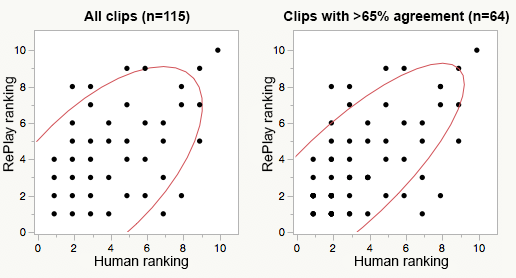
\includegraphics[width=\columnwidth]{liveclips/figures/agreement.png}
  \caption{Human ranking vs. RePlay ranking for all video clips (left), and all video clips with >65\% agreement among turkers (right). Note that there is more overall agreement between rankings in the subset on the right.}~\label{fig:liveclips_agreement}
\end{figure}

\begin{table}[b!]
\small
\centering
\textbf{All clips (n = 115)}
\vspace{5pt}
\begin{tabular}{l|llllllll}
\# Clips & 2    & 3 & 4 & 5   & 6    & 7    & 9    & 10   \\ \hline
\# Groups           & 18   & 5 & 2 & 1   & 1    & 1    & 2    & 2    \\
Mean $\rho$  & 0.11 & 0.3 & -0.2 & 0.6 & 0.09 & 0.54 & 0.21 & 0.48
\end{tabular}
\textbf{Clips with >65\% agreement (n = 64)}
\begin{tabular}{l|llll}
\# Clips & 2    & 3   & 4    & 5   \\ \hline
\# Groups           & 18   & 3   & 3    & 1   \\
Mean $\rho$  & 0.33 & 1.0 & 0.73 & 1.0
\end{tabular}
\caption{Average Spearman $\rho$ correlation between human ranking and RePlay ranking for all clips (top) and all clips with >65\% agreement among turkers (bottom), compared within each tool. ``\# Groups'' for column $i$ refers to the number of tools that have $i$ clips. Positive $\rho$ values indicate a positive correlation, with correlations above .2 considered weak, above .4 considered moderate, and above .6 considered strong.}
\label{table:agreement}
\end{table}

\section{Early user feedback}
The Mechanical Turk evaluation explored the viability of RePlay's ranking algorithm outside the context of an application. To get some initial user feedback on placing inspiring examples \textit{inside} an application, we recruited two casual Photoshop users, both male, to work on projects of their choice. They used Photoshop with all three interfaces enabled at once (on-demand search, ambient side panel, and contextual tooltips) (\autoref{fig:liveclips_photoshop}), and gave feedback while they worked.

Overall feedback was positive. Both participants found seeing video examples in the application useful and said that they wanted to see how others use tools and set parameters. The two participants differed in how they wanted to see examples. One participant preferred the tooltips, explaining that they were a nice level in between the on-demand search (which was easy to forget about) and the ambient panel (which they found distracting). They liked that if you happen to hover on a tool for an extra moment (which could happen by accident), it pops up and serves as a reminder that these examples exist, without taking away too much from the process. The other participant preferred the panel, and wanted to be able to refresh recommendations on demand and see a large variety of content. Both participants clicked on the videos and wanted to watch them in the browser where they could see them larger. 

This early user feedback is encouraging and shows the opportunity around embedding examples in the application.


\section{Discussion}

\subsection{Can we really predict what will be inspiring?}
The results from the ranking evaluation presented in the previous section should be taken with a grain of salt. The workers who participated in this study were not all users of creative software, and the video clips were presented out of context. The evaluation was intended as an initial baseline to determine whether RePlay's ranking algorithm can reasonably identify good clips. The subjective nature of the question workers were asked meant that we could not include a ``ground truth'' comparison to filter out lazy turkers. We did however enforce that the entire video clips played at least once before workers could select an answer.

Aside from the questions that using crowd-worker participants raises, the idea of ``inspiration'' is subjective and hard to predict. What one person finds inspiring another may not. Whether someone finds something inspiring could even change depending on the time at which they see it. Despite these challenges, we had reasonable agreement among workers overall; the average percent of agreement across all pairs of clips was 74\%, (SD 14.5). Even if Mechanical Turk workers \textit{were} a 100\% reliable source, we would still expect some disagreement, due to the subjective nature of the question.

The RePlay algorithm can reasonably identify clips that most workers agree are either good or bad. It is important to keep in mind that the main purpose for this algorithm is to address the ``cold start'' problem. Once people start using an interface with video examples, RePlay could continually improve the ranking algorithm based on user behaviour and preferences, exhibited through how much people interact with the videos. %There are other low-level features of clips identified by Lafreniere et al. \cite{Lafreniere2014} that could also be included in a ranking algorithm, such as whether a clip shows parameters being set, but we chose not to include these in the RePlay algorithm because it is likely that the \textit{content} of a video's artwork will be the main factor that determines its inspirational value. but this is a hard problem.

\subsection{How diverse should the set of examples be?}
Research on examples and creativity is rather divided regarding whether diverse examples that are distantly related to the user's task are better than a narrow set of examples that are more closely related to the user's task. Some work has shown that more diverse, far-off examples improve creativity by encouraging people to think more broadly and try new things \cite{Chan2011, Siangliulue2015a}, while other work has shown that similar examples are more useful as they are more relevant to the user \cite{Chan2015}. More recently, Benjamin et al. \cite{Benjamin2014} propose letting the user decide by providing an adjustable slider that determines the diversity of recommended examples, based on the idea that the need for more diverse or more similar examples may differ depending on where the user is in their process.

Another option could be to let users search by example, a feature that is now common in search engines. Rather than having to specify an exact query, users could provide an example video and ask for ``more like this''. However even in this case the diversity of results is an important factor to consider.

%let's cut this for now.It's good but not as connected to inspiration as the the previous sections, which work well together
%\subsection{How much information should recommendations show?}
%Prior research has shown the benefits of being transparent with users about how recommendations are chosen \cite{}. In our three interfaces, contextual tooltips are transparent by nature, as they show only clips of the selected tool. However the method for choosing clips in the search window and panel is currently rather opaque. It may be helpful to provide users with more detail regarding why a clip was chosen, for example because they used a certain tool recently. 

%More generally, providing users with enough information scent to make a quick but informed decision about whether they should give their attention to an example is important. This highlights a challenging trade-off in the design of contextual interfaces: showing users enough information without making it too costly to review this information \cite{?}. While there are many additional things that could be shown along with a video clip (a description of it, the audio transcript, the tools used in it, an overview of the task it shows, etc.) and existing methods for highlighting important activity within the clip (highlighting mouse movement or areas of change \cite{}, showing what keys are being pressed when \cite{}), incorporating all of this information would quickly become overwhelming. Prior work has shown that a brief text description can help users efficiently scan a set of video clips \cite{}; this may be a good starting point.
\section{Limitations \& Future Work}
This chapter presented initial work exploring ways to bring inspiring examples into the creative process, and a new type of content from which to draw such examples: creative live stream videos. We provide suggestive results that our algorithm can select potentially inspiring clips, and some initial user feedback on our prototype interfaces indicating that this is a promising avenue for future work. Rather than conduct a rigorous controlled study (which is difficult and often inappropriate for evaluating goals like creativity and inspiration \cite{Shneiderman2007}), this chapter aims to introduce this space and lay out the possibilities for future work to explore. In this section, we discuss a few main directions for such work.

\subsection{More Robust Segmentation and Change Ranking}
Our current methods for detecting visual change use simple computer vision approaches, and exhibited some failure cases. We have yet to try more sophisticated deep learning methods to segment this data but this is a promising direction of future work that could help improve the classification of panning, zooming, and parameter setting. Having more robust and available usage data could also improve the detection of such features. For example, Lafreniere \textit{et al.} \cite{Lafreniere2014} used instrumented software to gather both videos and detailed usage, which allowed them to calculate visual change directly by counting the number of pixels on the artist's document that change during a video clip. As of recently, streamers on Behance (\href{https://behance.net/live}{\nolinkurl{behance.net/live}}) can use a plugin that logs their command usage while they stream in creative software. This data can be used to segment live stream archives \cite{Fraser2020}, but such segmentations would still benefit from logs or analysis of visual and spatial information.

In addition, to make use of the large amount of video content that already exists online with no available telemetry, a deep learning system could be trained on those videos that do have usage data, and then applied to videos that do not.

\subsection{Making Use of Audio and Chat Logs}
Live streamed videos come with additional data that this work did not make use of: audio in the form of the streamer's narration and responses to questions (which can be transcribed to text) and chat logs from viewers of the stream. Making use of audio narration in software tutorial videos is an open problem \cite{Chi2012} as narrations don't always align exactly with the artist's actions. Live streamed videos have a similar problem that is exacerbated by the fact that artists are not always narrating what they are doing; sometimes they are answering questions from the chat and other times they are simply talking about unrelated things as they work. Future work should explore ways to detect when those different types of narration are occurring, and make use of their content as appropriate, for example highlighting moments where artists answer questions, or building a mapping of ways in which artists describe their software actions in natural language.

Chat logs can also be a useful data source to include in future work. Though the content of live chats tends to be very noisy, especially on popular channels \cite{Hamilton2014}, the frequency of chat posts at a given time can indicate exciting or interesting moments \cite{Pan2016}. Chat post frequency could therefore be used as another criteria for ranking clips.

\subsection{Other Ways to Generate Short Clips from Long Videos}
This work focused on generating tool-based clips, inspired by prior work \cite{Grossman2010a, Lafreniere2014} and the natural mapping between tool use and user behaviour. However, while tool-focused clips are good for showing users how a tool works \cite{Grossman2010a}, they may not be the most inspirational types of clips one can generate from long videos. Other methods could include breaking videos into higher level sub-tasks (based on pauses in tool activity and narration content), or extracting clips where the artist describes a particular technique or answers a question. As one of the exciting parts of watching a live stream is seeing an artist go from a blank canvas to a finished work, another option could be to shorten the entire video down to a short summary. This could be done by removing sections where the artist takes pauses, talks with no actions, and switches applications; and by adapting existing techniques for creating short video summaries from long videos (\textit{e.g.}, \cite{Truong2007}). 

\section{Conclusion}
This chapter explored a growing form of creative videos very different from traditional tutorials: live streams. We found that creative live streams are a good source of both learning and inspiration, and introduced an approach for bringing inspiration into the context of creative software users' workflows. 

RePlay, ReMap, and LiveClips all leveraged \textbf{visual media} in the form of screencast videos for providing contextual support towards understanding creative processes. But for users who just want to get a task done without spending time on the individual steps required, videos can be too tedious and detailed. The next two chapters explore how two different types of resource -- \textbf{executable code} and \textbf{written text} -- can help people quickly and easily achieve creative outcomes.


\section{Acknowledgements}
We thank Tricia Ngoon, Kandarp Khandwala, and Nicolas La-polla for their help with live stream analysis, and our study participants for their insights. This work was supported in part by NSERC, Adobe Research, and NSF award \#1735234.

This chapter, in part, includes portions of material as it appears in \textit{Sharing the Studio: How Creative Livestreaming can Inspire, Educate, and Engage} by C. Ailie Fraser, Joy O. Kim, Alison Thornsberry, Scott Klemmer, and Mira Dontcheva in the Proceedings of the 2019 on Creativity and Cognition (C\&C '19). The dissertation author was the primary investigator and author of this paper.

This chapter, in part, includes portions of material coauthored with Andy Edmonds and Mira Dontcheva. The dissertation author was the primary investigator and author of this material.
